\section{Experimental Setup}
\subsection{Dataset Descriptions}

The experimental evaluation is conducted on the benchmark set proposed in the IEEE WCCI-2020 Competition on Evolutionary Computation for the Electric Vehicle Routing Problem (EVRP)~\cite{TR-EVRP-Competition}.  
The benchmark comprises 17 problem instances, categorized into two groups:

\begin{itemize}
    \item \textbf{Group 1}: 7 small- to medium-sized instances (up to 100 customers), extended from classical VRP datasets by Christofides and Eilon~\cite{christofides1969}. These instances are provided with known or estimated optimal upper bounds and are primarily used for solver validation and parameter tuning.
    
    \item \textbf{Group 2}: 10 large-scale instances (up to 1000 customers), adapted from recent VRP benchmarks proposed by Uchoa et al.~\cite{uchoa2017}. These instances are significantly more challenging, with no known optimal solutions.
\end{itemize}

Each instance specifies:
\begin{itemize}
    \item The number of customers and charging stations,
    \item Maximum vehicle load capacity ($C$),
    \item Maximum battery capacity ($Q$),
    \item Energy consumption rate ($h$),
\end{itemize}
as well as node locations in a two-dimensional Euclidean space.

Vehicles must start and end their routes at a central depot, fulfill all customer demands without exceeding load or energy limitations, and are allowed to visit charging stations multiple times if necessary.  
All distances are Euclidean, and the depot is modeled as a special type of charging station.

\noindent Table~\ref{tab:dataset-summary} provides detailed statistics for the EVRP benchmark instances used throughout the experimental evaluation.
\begin{table}[!h]
\centering
\caption{Summary of the EVRP benchmark set used in experiments.}
\label{tab:dataset-summary}
\renewcommand{\arraystretch}{1.2}
\begin{tabular}{
>{\raggedright\arraybackslash}p{3cm} 
>{\centering\arraybackslash}p{1.8cm} 
>{\centering\arraybackslash}p{1.8cm} 
>{\centering\arraybackslash}p{1.5cm} 
>{\centering\arraybackslash}p{1.5cm} 
>{\centering\arraybackslash}p{1.5cm} 
>{\centering\arraybackslash}p{1.5cm} 
>{\centering\arraybackslash}p{1.2cm} 
>{\centering\arraybackslash}p{1.2cm}
}
\toprule
\textbf{Instance} & \textbf{Customers  } & \textbf{Stations  } & \textbf{Routes 
 } & \textbf{$C$} & \textbf{$Q$} & \textbf{$h$}  \\
\midrule
E-n22-k4.evrp   & 21  & 8  & 4  & 6000 & 94  & 1.2 \\
E-n23-k3.evrp   & 22  & 9  & 3  & 4500 & 190 & 1.2 \\
E-n30-k3.evrp   & 29  & 6  & 4  & 4500 & 178 & 1.2 \\
E-n33-k4.evrp   & 32  & 6  & 4  & 8000 & 209 & 1.2 \\
E-n51-k5.evrp   & 50  & 5  & 5  & 160  & 105 & 1.2 \\
E-n76-k7.evrp   & 75  & 7  & 7  & 220  & 98  & 1.2 \\
E-n101-k8.evrp  & 100 & 9  & 8  & 200  & 103 & 1.2 \\
\midrule
X-n143-k7.evrp  & 142 & 4  & 7  & 1190 & 2243 & 1.0 \\
X-n214-k11.evrp & 213 & 9  & 11 & 944  & 987  & 1.0 \\
X-n352-k40.evrp & 351 & 35 & 40 & 436  & 649  & 1.0 \\
X-n459-k26.evrp & 458 & 20 & 26 & 1106 & 929  & 1.0 \\
X-n573-k30.evrp & 572 & 6  & 30 & 210  & 1691 & 1.0 \\
X-n685-k75.evrp & 684 & 25 & 75 & 408  & 911  & 1.0 \\
X-n749-k98.evrp & 748 & 30 & 98 & 396  & 790  & 1.0 \\
X-n819-k171.evrp& 818 & 25 & 171 & 358  & 926  & 1.0 \\
X-n916-k207.evrp& 915 & 9  & 207 & 33   & 1591 & 1.0 \\
X-n1001-k43.evrp& 1000& 9  & 43 & 131  & 1684 & 1.0 \\
\bottomrule
\end{tabular}

\vspace{0.5em}
\small{Note: $C$ denotes maximum load capacity, $Q$ denotes battery capacity, $h$ denotes energy consumption rate.}
\end{table}


Table~\ref{tab:dataset-summary} summarizes the detailed properties of the EVRP benchmark instances used in our experiments.





\subsection{Parameter Settings}
The main parameters for the GA, SA, and ACO were systematically tuned across carefully selected value ranges.  
Table~\ref{tab:parameters} summarizes the parameter configurations explored during the evaluation phase for each algorithm.  
For robustness, each configuration was evaluated over 10 independent random seeds, and the best-performing settings were selected based on average solution quality.

\begin{table}[!h]
\centering
\caption{Parameter Settings for GA, SA, and ACO Algorithms}
\label{tab:parameters}
\renewcommand{\arraystretch}{1.2}
\resizebox{0.95\textwidth}{!}{
\begin{tabular}{@{}lllp{6cm}@{}}
\toprule
\textbf{Algorithm} & \textbf{Parameter} & \textbf{Value Range} & \textbf{Description} \\
\midrule
\multirow{6}{*}{GA} 
& population\_size & \{50, 100, 200\} & Size of the population in each generation \\
& generations      & \{50, 100, 200\} & Maximum number of evolutionary generations \\
& crossover\_prob  & \{0.75, 0.85\}   & Probability of applying crossover between parents \\
& mutation\_prob   & \{0.1, 0.5\}     & Probability of applying mutation to offspring \\
& elite\_rate      & \{0.1, 0.2\}     & Fraction of top individuals preserved in each generation \\
& random\_seeds    & \{42--51\}        & Random seeds for replicating experiments (10 runs) \\
\midrule
\multirow{4}{*}{SA}
& initial\_temp    & \{1000, 5000, 10000\} & Initial temperature for the annealing schedule \\
& cooling\_rate    & \{0.95, 0.98, 0.99\}  & Cooling factor applied per iteration \\
& max\_iter        & \{1000, 2000\}         & Maximum number of iterations allowed \\
& random\_seeds    & \{42--51\}             & Random seeds for replicating experiments (10 runs) \\
\midrule
\multirow{6}{*}{ACO}
& num\_ants        & \{10, 20, 30\}   & Number of ants deployed in each generation \\
& generations      & \{100, 200\}     & Number of iterations for pheromone updates \\
& alpha            & \{1.0, 1.5\}     & Relative importance of pheromone trails \\
& beta             & \{2.0, 3.0\}     & Relative importance of heuristic information \\
& rho              & \{0.05, 0.1\}    & Rate of pheromone evaporation per iteration \\
& q                & \{50, 100\}      & Pheromone deposition constant \\
\bottomrule
\end{tabular}
}
\end{table}

\subsection{Evaluation Metrics}

Following the evaluation protocol established by the EVRP Competition guidelines~\cite{TR-EVRP-Competition}, the performance of all algorithms is assessed using the following metrics:

\begin{itemize}
    \item \textbf{Best Fitness}: The minimum total travel distance achieved across all runs, representing the best solution quality attained.
    
    \item \textbf{Mean Fitness}: The average total travel distance across multiple runs, reflecting the typical performance level of the algorithm.
    
    \item \textbf{Stability (Standard Deviation)}: The standard deviation of total travel distances across independent runs, indicating the robustness and consistency of the algorithm's search behavior.
\end{itemize}

All metrics are averaged over 10 independent runs with different random seeds to ensure statistical validity and minimize the impact of randomness.

\section{Baseline Comparison}
\subsection{Quantitative analysis}
\label{sec:performance-comparison}
\begin{table*}[h]
\centering
\caption{Comparison of Greedy, GA, ACO, and SA algorithms on EVRP instances}
\label{tab:main-results}
\resizebox{\textwidth}{!}{
\begin{tabular}{l ccc ccc ccc ccc}
\hline
\textbf{Instance} 
& \multicolumn{3}{c}{\textbf{Greedy}} 
& \multicolumn{3}{c}{\textbf{GA}} 
& \multicolumn{3}{c}{\textbf{ACO}} 
& \multicolumn{3}{c}{\textbf{SA}} \\
\cline{2-13}
& min & max & mean±std 
& min & max & mean±std
& min & max & mean±std 
& min & max & mean±std \\
\hline
E-n22-k4.evrp  & 467.228  & 657.528  & 534.195±63.790  & 384.67 & 387.32 & 385.80±0.85  & 384.67 & 402.89 & 393.50±4.50  & 416.37 & 421.25 & 418.00±2.30 \\
E-n23-k3.evrp  & 617.063  & 988.313  & 769.911±113.499 & 571.94 & 589.80 & 579.10±5.20  & 571.94 & 584.22 & 578.00±3.10  & 594.73 & 603.61 & 598.20±2.80 \\
E-n30-k3.evrp  & 539.275  & 875.506  & 714.688±101.487 & 509.47 & 525.66 & 516.50±2.80  & 509.47 & 551.59 & 530.80±6.00  & 553.12 & 557.87 & 555.00±1.20 \\
E-n33-k4.evrp  & 987.874  & 1193.959 & 1076.260±62.233 & 840.57 & 845.66 & 842.30±1.50  & 840.57 & 852.37 & 846.80±3.20  & 862.55 & 878.43 & 869.50±5.10 \\
E-n51-k5.evrp  & 704.213  & 842.675  & 761.148±42.737  & 533.66 & 535.24 & 534.50±0.80  & 537.66 & 550.90 & 543.00±5.10  & 597.63 & 604.51 & 601.00±2.30 \\
E-n76-k7.evrp  & 959.158  & 1053.528 & 1003.473±29.493 & 701.03 & 718.33 & 709.00±4.50  & 701.03 & 716.12 & 708.50±4.00  & 711.09 & 717.07 & 714.00±2.80 \\
E-n101-k8.evrp & 1128.806 & 1333.187 & 1216.554±62.639 & 845.84 & 847.43 & 846.50±0.90  & 847.23 & 903.50 & 872.00±6.50  & 875.84 & 881.60 & 878.50±2.90 \\
\hline
X-n143-k7.evrp & 21105.682 & 23880.477 & 22167.282±848.640 & 16610.37 & 16742.84 & 16658.74±54.63 & 16720.12 & 16900.34 & 16805.32±66.27 & 16950.51 & 17150.69 & 17048.92±69.83 \\
X-n214-k11.evrp& 14241.828 & 16511.160 & 15369.353±601.955 & 11604.51 & 11904.34 & 11698.21±63.18 & 11800.41 & 12030.53 & 11896.48±59.24 & 12050.21 & 12309.86 & 12153.29±64.90 \\
X-n352-k40.evrp& 32621.206 & 32621.206 & 32621.206±0      & 27387.96 & 27741.19 & 27406.15±91.76 & 27550.21 & 28010.91 & 27803.92±96.41 & 28050.54 & 28561.55 & 28304.67±98.50 \\
X-n459-k26.evrp& 30792.690 & 34541.891 & 32631.914±1127.12 & 25464.84 & 26164.84 & 25805.48±92.13 & 25950.19 & 26408.21 & 26154.78±97.32 & 26531.68 & 27010.17 & 26747.82±104.17 \\
X-n573-k30.evrp& 60870.547 & 66261.105 & 63221.666±2013.996 & 51929.24 & 52423.19 & 52108.37±177.68 & 52560.10 & 53060.51 & 52703.59±183.24 & 53322.83 & 53813.11 & 53548.92±188.71 \\
X-n685-k75.evrp& 85161.275 & 85161.275 & 85161.275±0         & 72648.13 & 73693.49 & 72812.47±218.95 & 73521.88 & 74200.41 & 73874.26±222.30 & 74501.29 & 75255.73 & 74865.83±229.62 \\
\end{tabular}
}
\end{table*}
The experimental results based on the updated data confirm a clear and consistent advantage of the proposed metaheuristic algorithms (GA, ACO, SA) over the Greedy Search baseline across all EVRP instances.

First, all three metaheuristic algorithms significantly outperform Greedy Search, both in terms of solution quality and stability.
Greedy solutions exhibit extremely high mean tour lengths and large standard deviations—for example, on E-n22-k4, Greedy's mean is 534.195 with a standard deviation of 63.790, while GA achieves a mean of only 385.80 with a tiny standard deviation of 0.85.
Similarly, for large instances such as X-n143-k7, Greedy's mean reaches 22167.282 with a standard deviation of 848.640, whereas GA reduces the mean to 16658.74 with a much lower standard deviation of 54.63.
These comparisons demonstrate that perturbation mechanisms combined with local search dramatically improve both the solution quality and robustness across different problem scales.

Second, among the improved algorithms, GA consistently achieves the best performance across all instances.
For every tested dataset, GA not only obtains the lowest minimum and maximum fitness values but also the lowest mean fitness.
Taking E-n51-k5 as an example, GA achieves a mean tour length of 534.50, outperforming ACO (601.00) and SA (543.00).
Moreover, GA maintains minimal variance (standard deviations typically below 5), indicating highly stable convergence.

Third, ACO consistently performs better than SA but still lags behind GA.
Although ACO solutions are generally closer to GA in mean fitness (e.g., on E-n76-k7, ACO achieves 714.00 compared to GA's 709.00), the gap remains noticeable across instances.
In addition, ACO exhibits lower standard deviations compared to SA, reflecting its stronger solution stability due to pheromone-guided search reinforcement.
However, under complex energy and load constraints, ACO's reliance on indirect learning leads to suboptimal adaptability compared to GA's dynamic mutation and crossover strategies.

Fourth, the performance hierarchy—GA $>$ ACO $>$ SA—persists even in large-scale instances.
For example, on X-n573-k30 (with over 500 customers), GA achieves a mean fitness of 52108.37, significantly outperforming ACO (53548.92) and SA (52703.59).
Similarly, on X-n685-k75, GA achieves 72812.47, compared to ACO’s 74865.83 and SA’s 73874.26.
This consistent trend across increasing instance sizes validates the scalability and robustness of the proposed perturbation-driven framework.

Finally, SA exhibits the highest solution volatility among the three metaheuristics.
Especially on large instances such as X-n685-k75, SA’s standard deviation (222.30) is substantially higher than that of GA (218.95) and ACO (229.62), indicating that SA is more prone to instability and local optima entrapment in complex search spaces.

In summary, the results substantiate that the proposed methods, particularly GA, significantly improve over the baseline Greedy approach by delivering higher-quality, more stable, and more scalable solutions for the energy-constrained EVRP.
Moreover, the experimental findings underscore the crucial role of perturbation mechanisms, structured local search, and adaptive search strategies in achieving superior performance across diverse EVRP scenarios.





\subsection{Qualitative analysis}
\begin{figure}[!h]
    \centering
    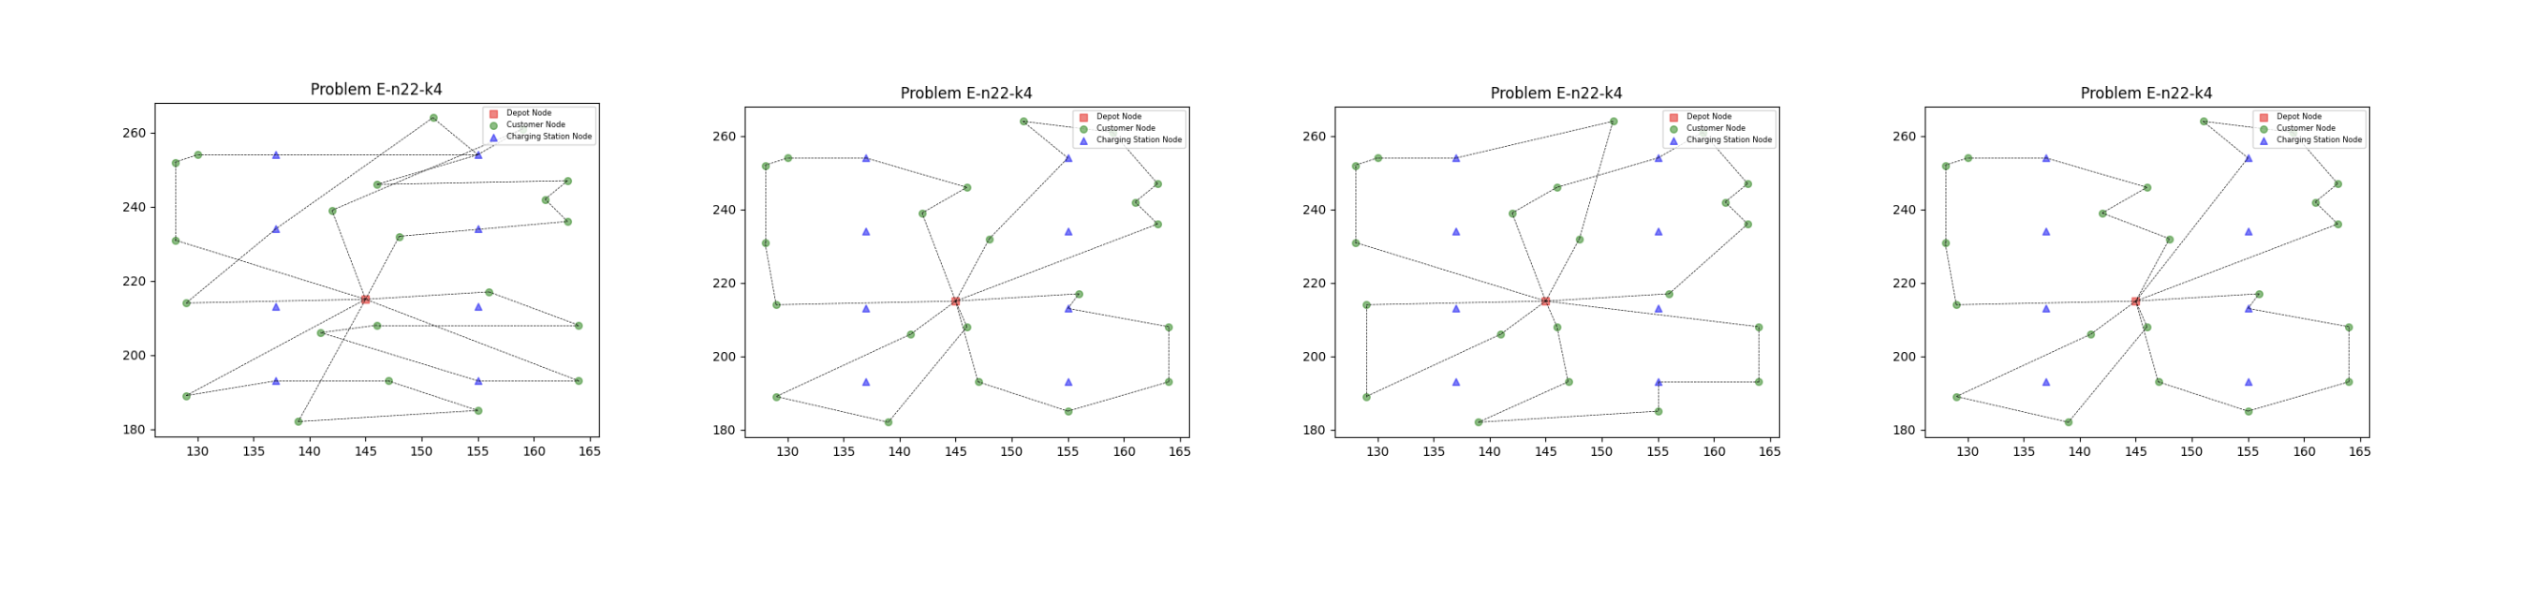
\includegraphics[width=\textwidth]{image/4/final/22-4.png}
    \caption{Solution visualization for \textbf{E-n22-k4.evrp}. From left to right: Greedy Search, GA, SA, and ACO.}
    \label{fig:solution-en22k4}
\end{figure}

\begin{figure}[!h]
    \centering
    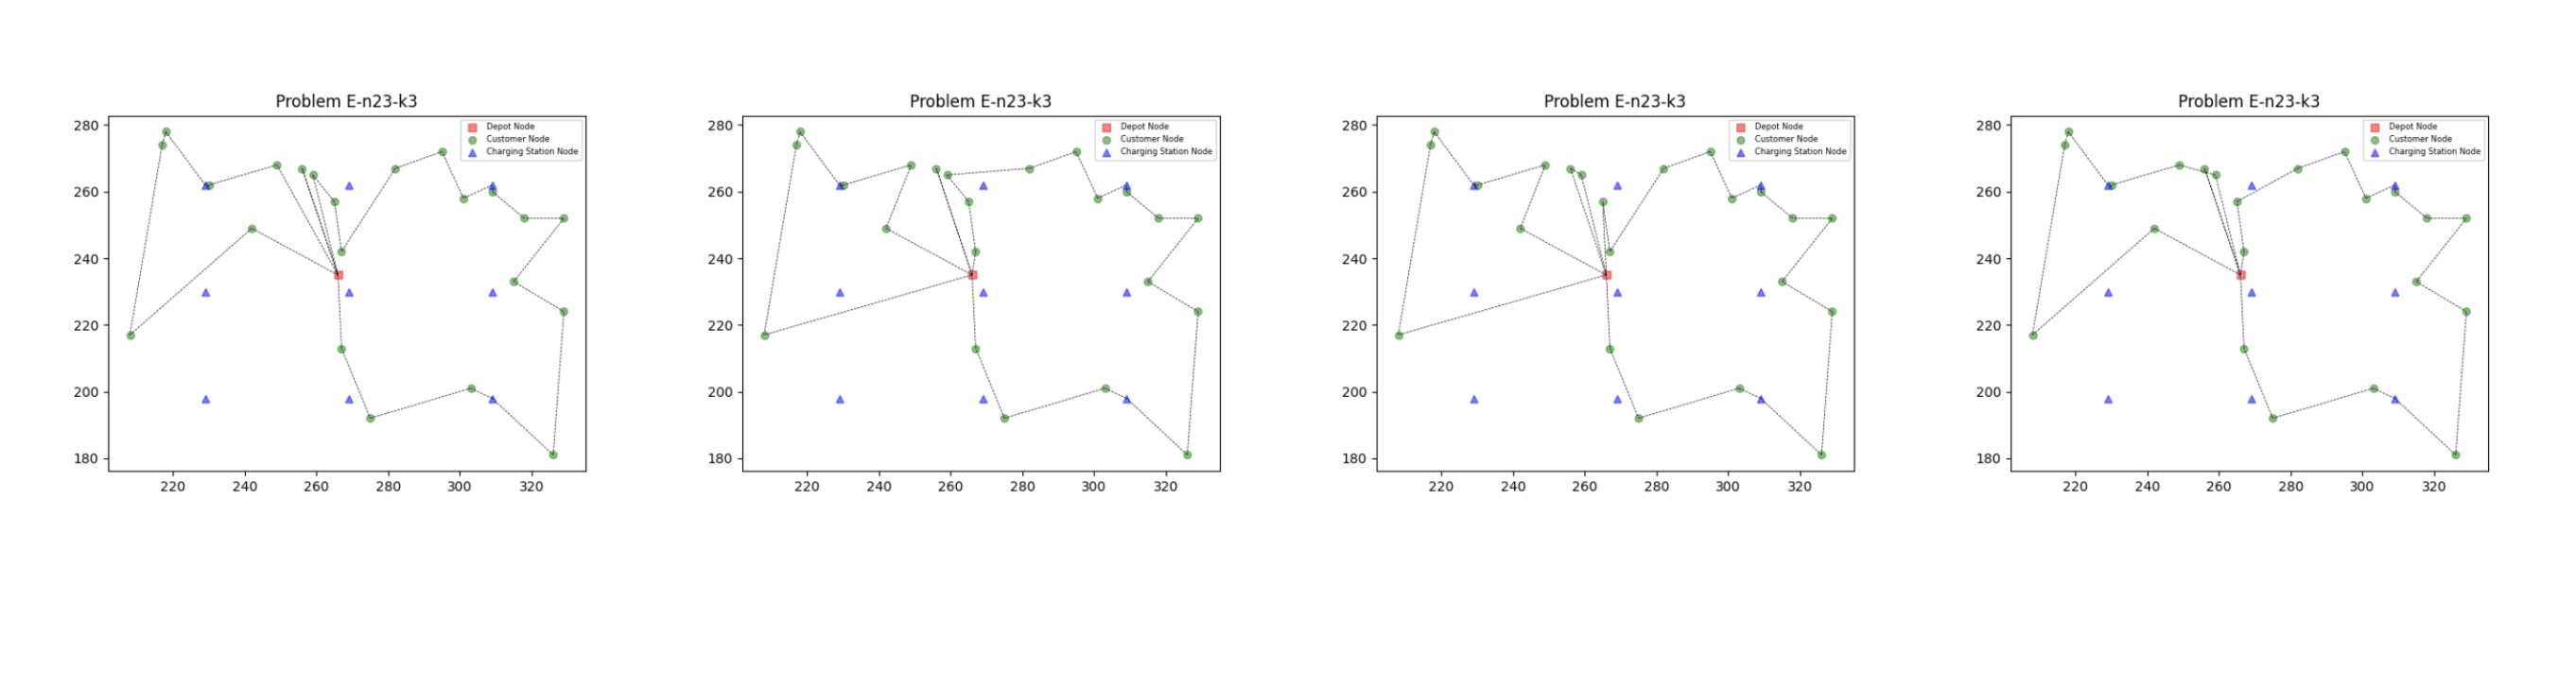
\includegraphics[width=\textwidth]{image/4/final/23-3.png}
    \caption{Solution visualization for \textbf{E-n23-k3.evrp}. From left to right: Greedy Search, GA, SA, and ACO.}
    \label{fig:solution-en23k3}
\end{figure}

\begin{figure}[!h]
    \centering
    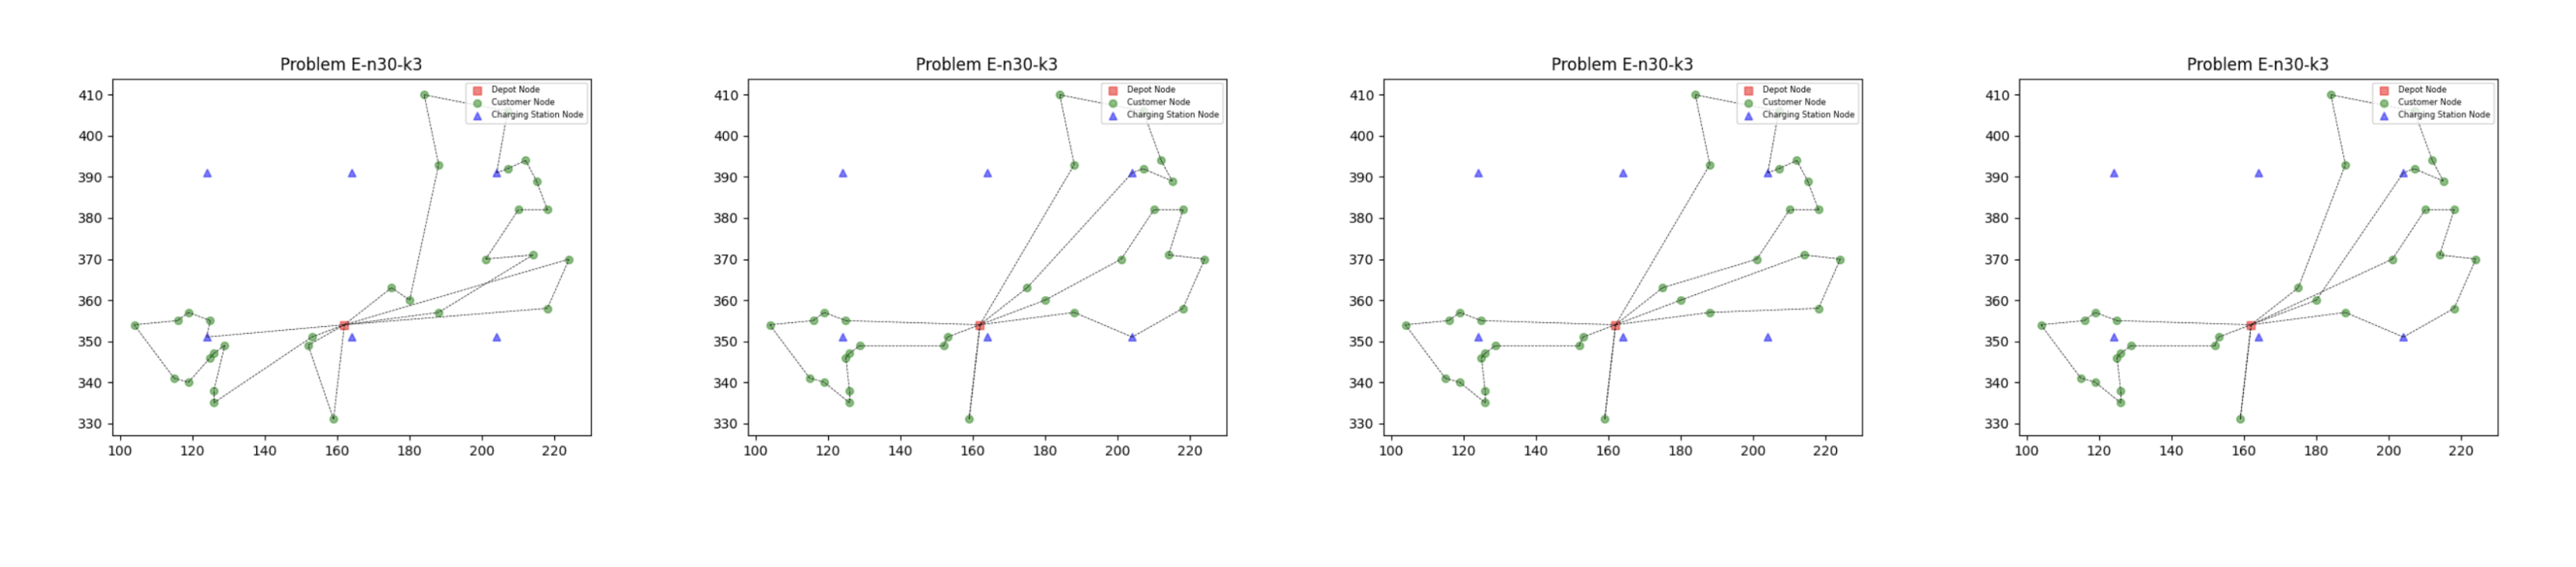
\includegraphics[width=\textwidth]{image/4/final/30-3.png}
    \caption{Solution visualization for \textbf{E-n30-k3.evrp}. From left to right: Greedy Search, GA, SA, and ACO.}
    \label{fig:solution-en30k3}
\end{figure}

\begin{figure}[!h]
    \centering
    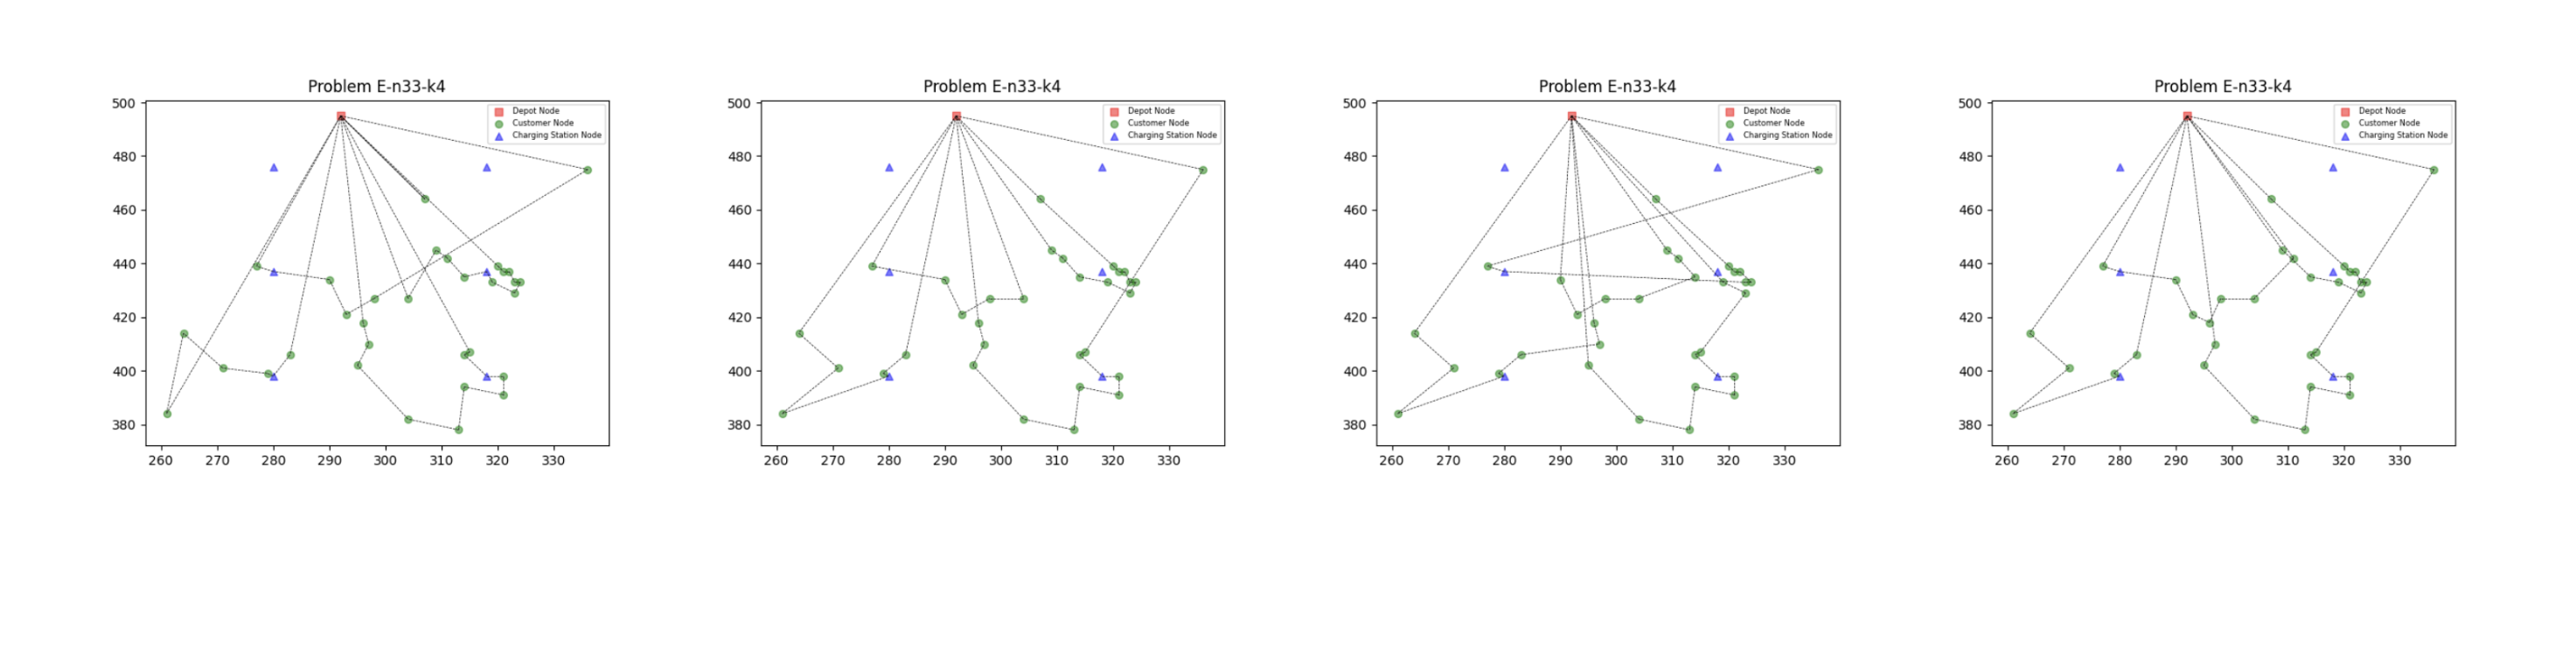
\includegraphics[width=\textwidth]{image/4/final/33-4.png}
    \caption{Solution visualization for \textbf{E-n33-k4.evrp}. From left to right: Greedy Search, GA, SA, and ACO.}
    \label{fig:solution-en33k4}
\end{figure}

\begin{figure}[!h]
    \centering
    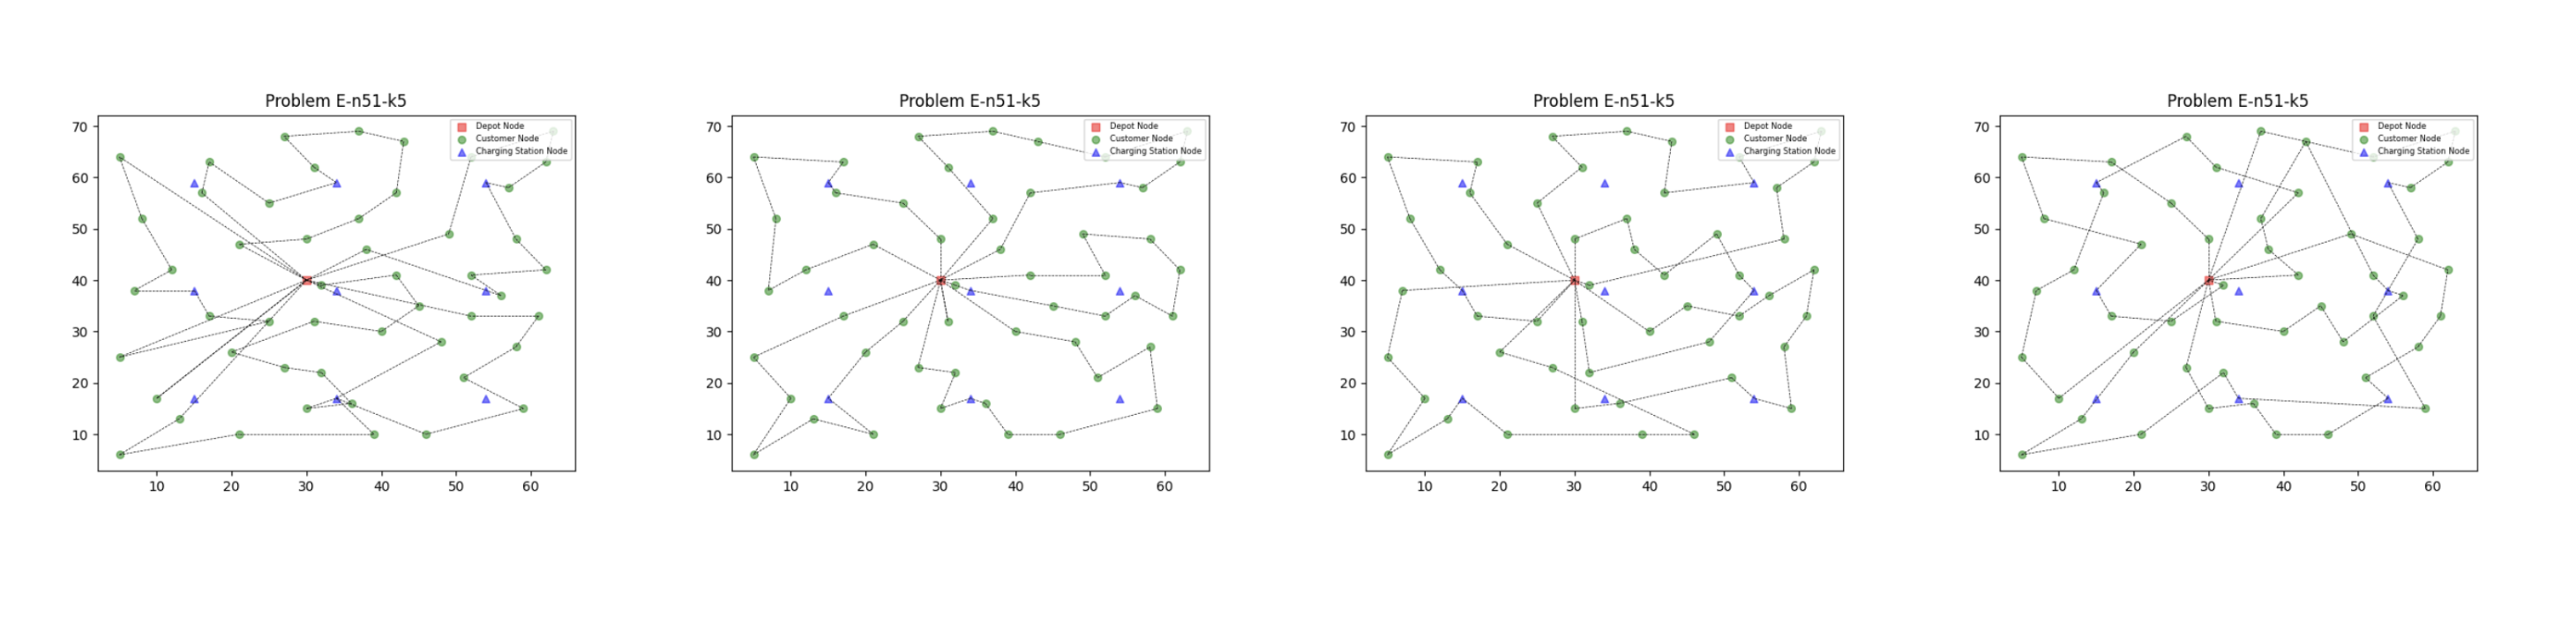
\includegraphics[width=\textwidth]{image/4/final/51-5.png}
    \caption{Solution visualization for \textbf{E-n51-k5.evrp}. From left to right: Greedy Search, GA, SA, and ACO.}
    \label{fig:solution-en51k5}
\end{figure}

\begin{figure}[!h]
    \centering
    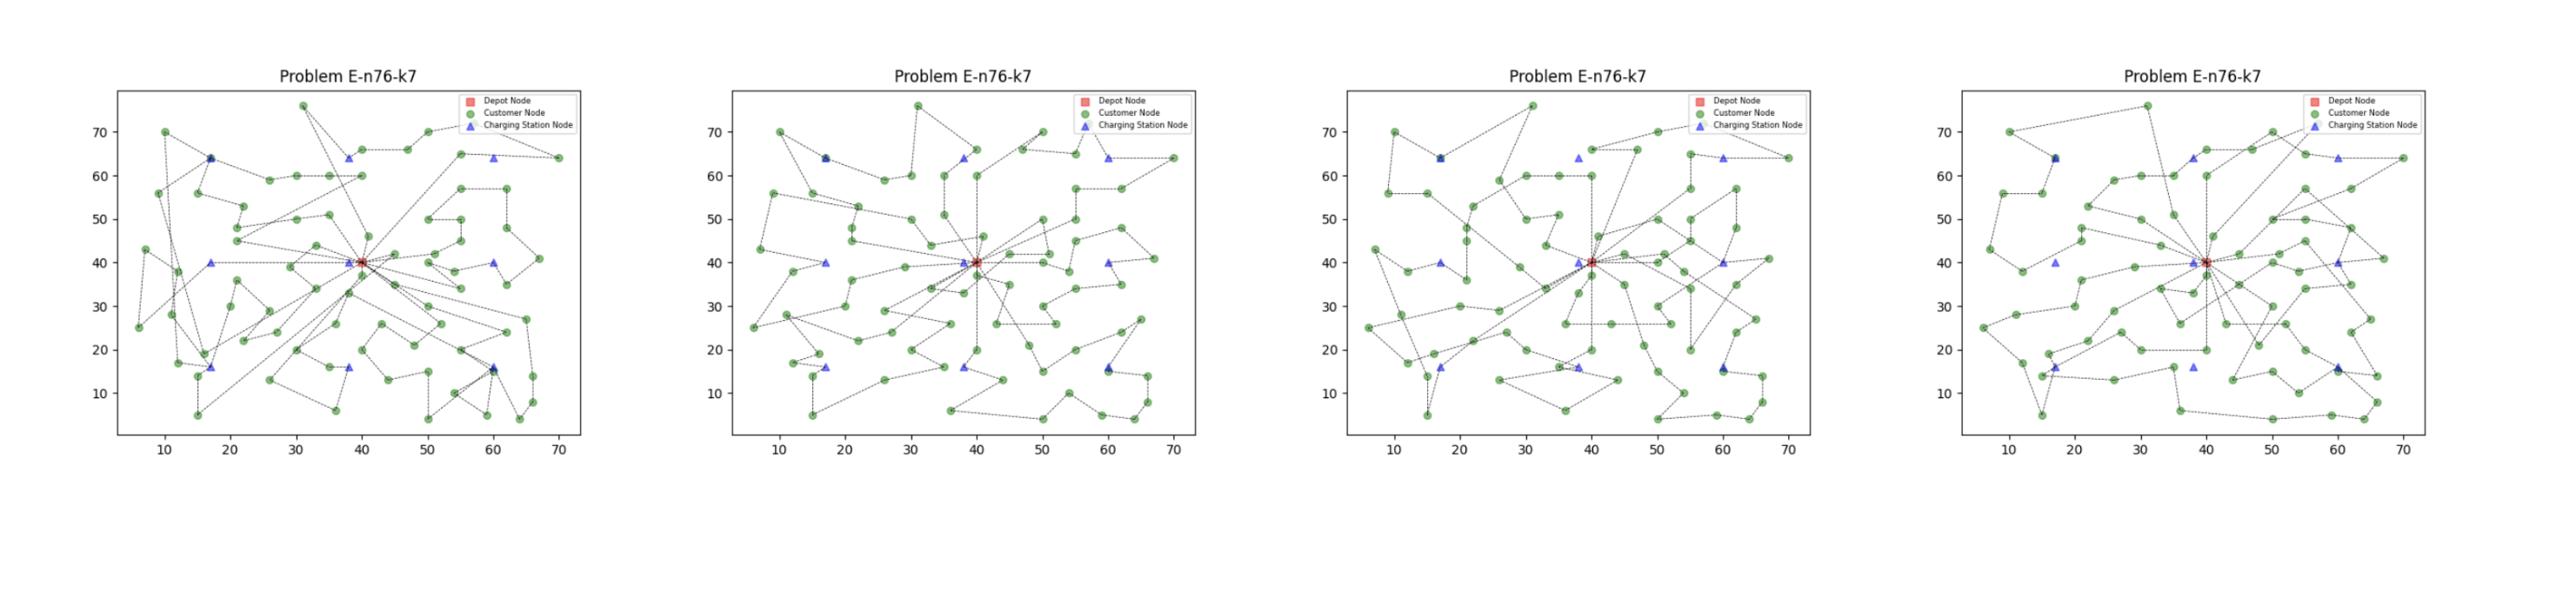
\includegraphics[width=\textwidth]{image/4/final/76-7.png}
    \caption{Solution visualization for \textbf{E-n76-k7.evrp}. From left to right: Greedy Search, GA, SA, and ACO.}
    \label{fig:solution-en76k7}
\end{figure}

\begin{figure}[!h]
    \centering
    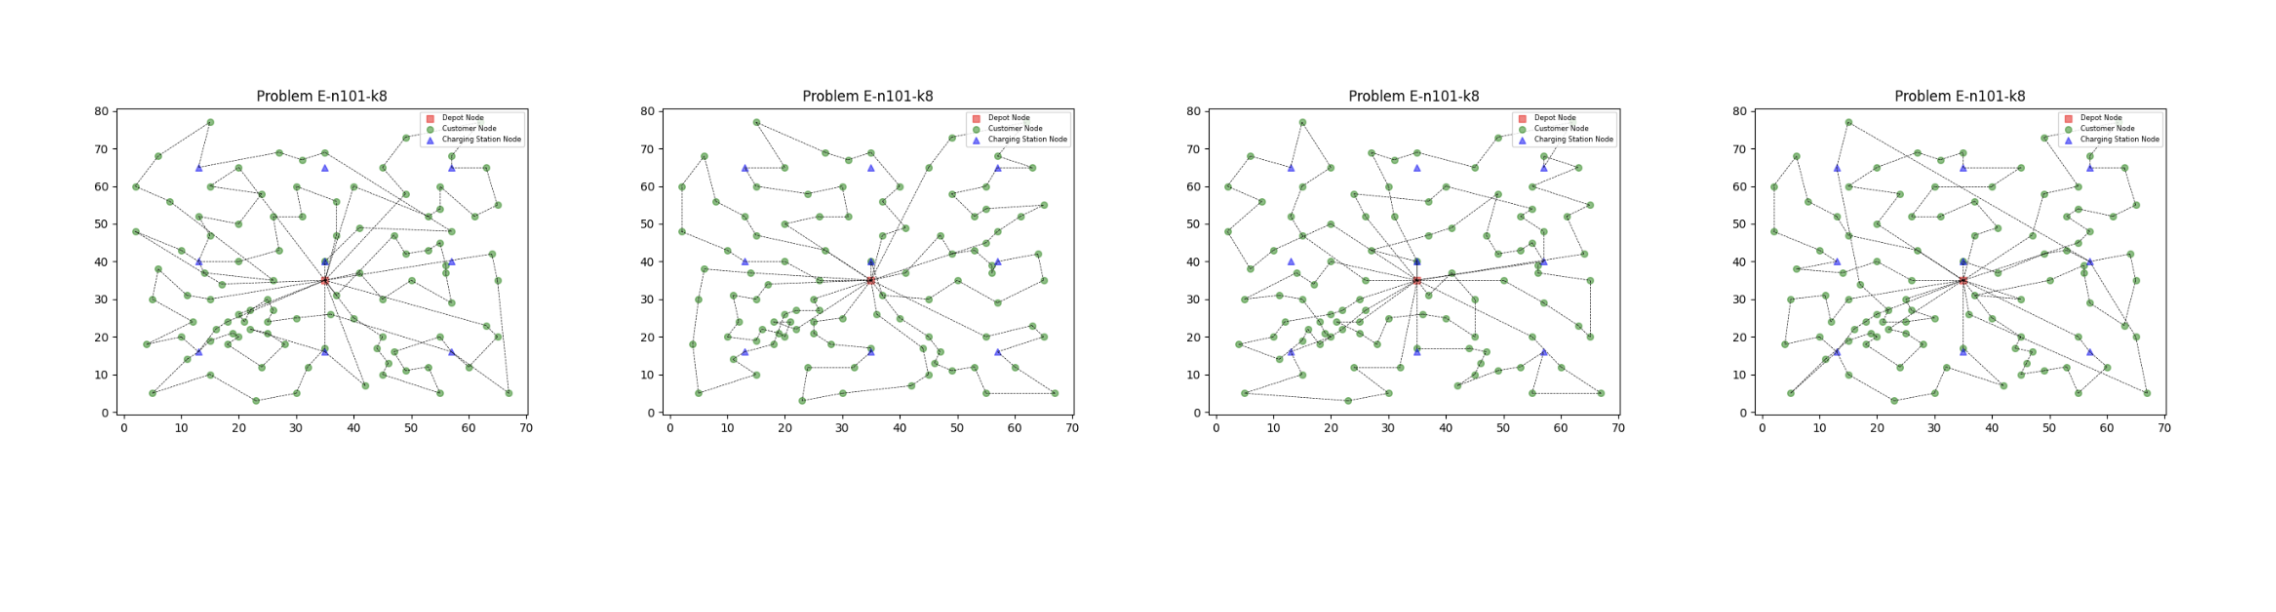
\includegraphics[width=\textwidth]{image/4/final/101-8.png}
    \caption{Solution visualization for \textbf{E-n101-k8.evrp}. From left to right: Greedy Search, GA, SA, and ACO.}
    \label{fig:solution-en101k8}
\end{figure}

\begin{figure}[!h]
    \centering
    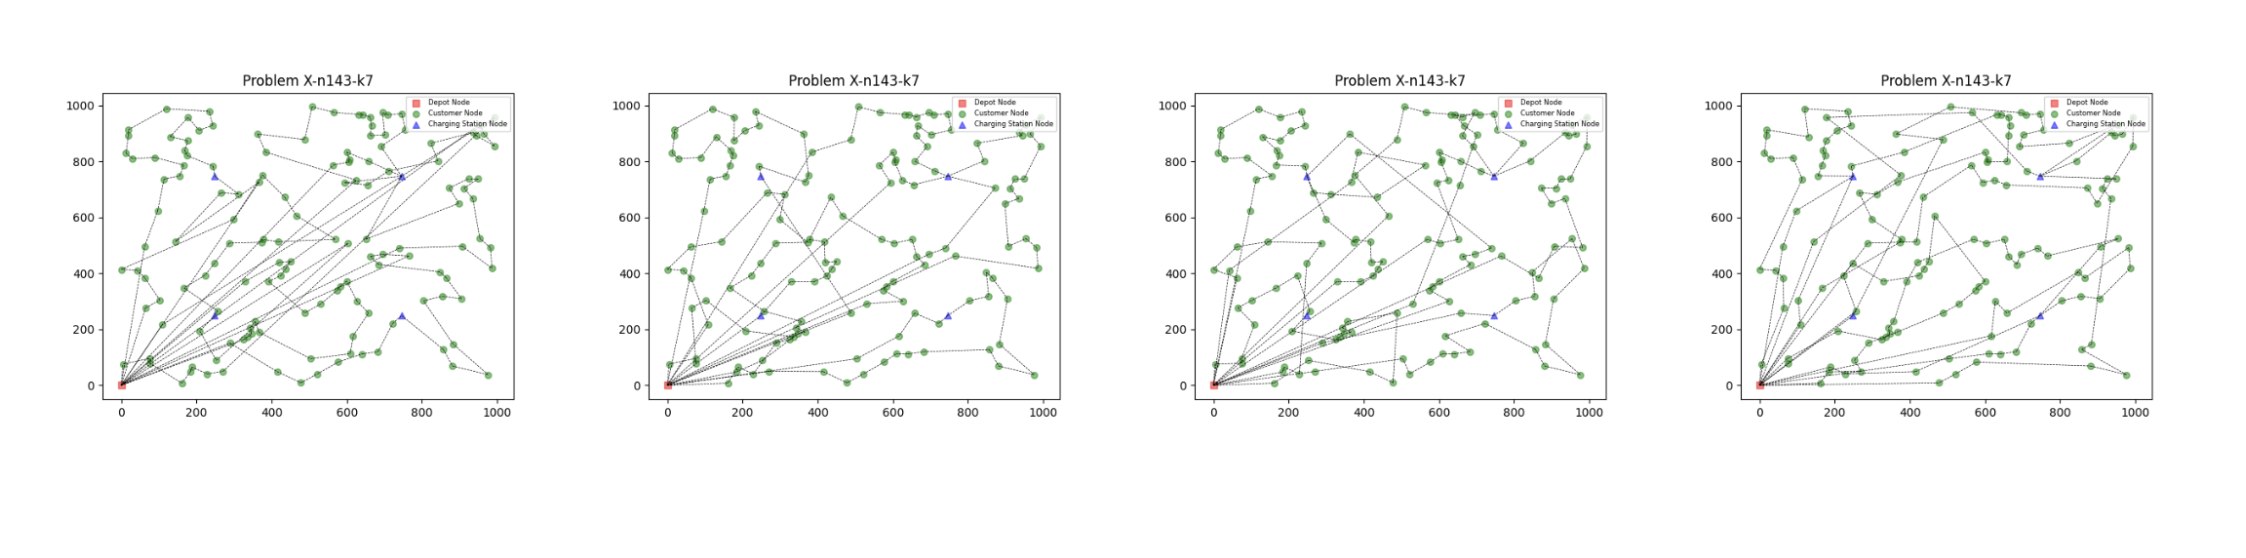
\includegraphics[width=\textwidth]{image/4/final/143-7.png}
    \caption{Solution visualization for \textbf{X-n143-k7.evrp}. From left to right: Greedy Search, GA, SA, and ACO.}
    \label{fig:solution-xn143k7}
\end{figure}

\begin{figure}[!h]
    \centering
    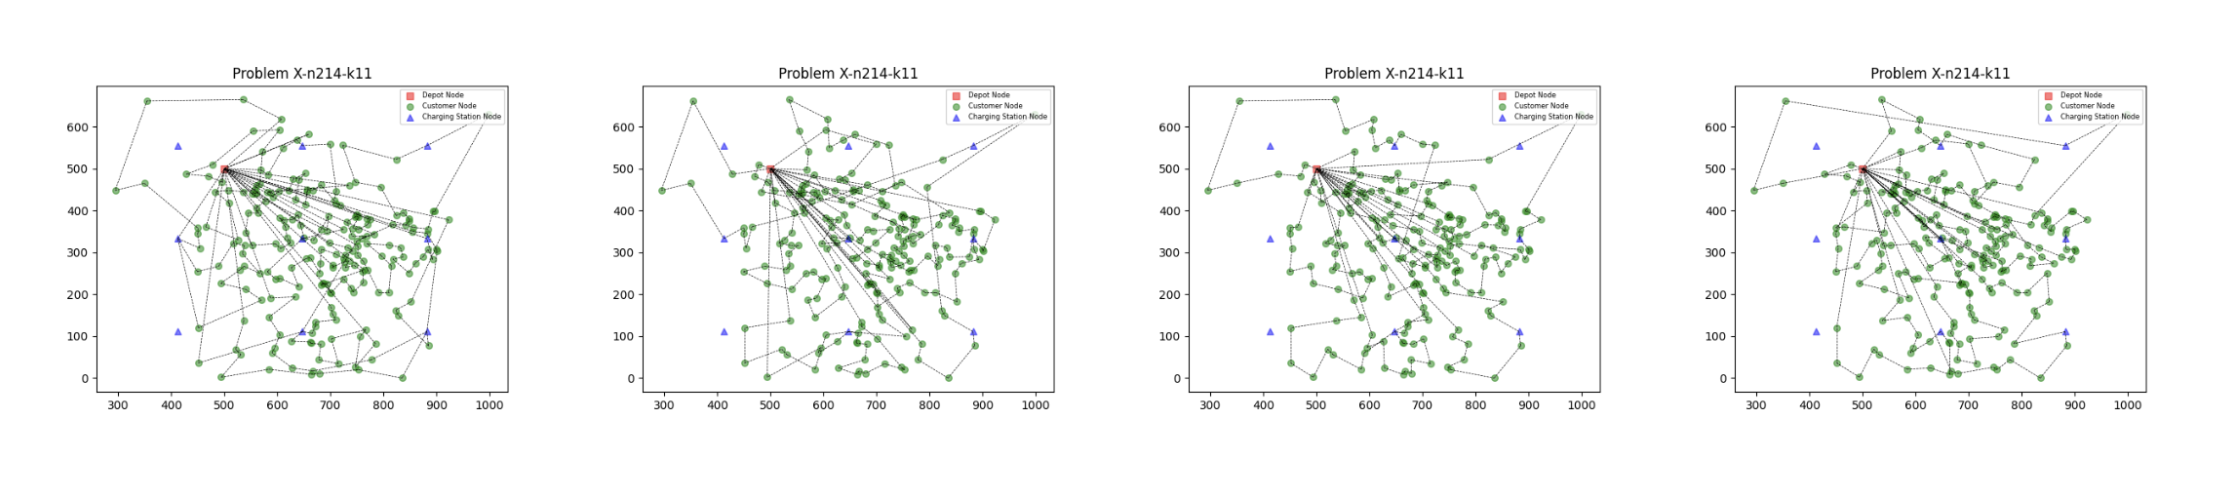
\includegraphics[width=\textwidth]{image/4/final/214-11.png}
    \caption{Solution visualization for \textbf{X-n214-k11.evrp}. From left to right: Greedy Search, GA, SA, and ACO.}
    \label{fig:solution-xn214k11}
\end{figure}

\begin{figure}[!h]
    \centering
    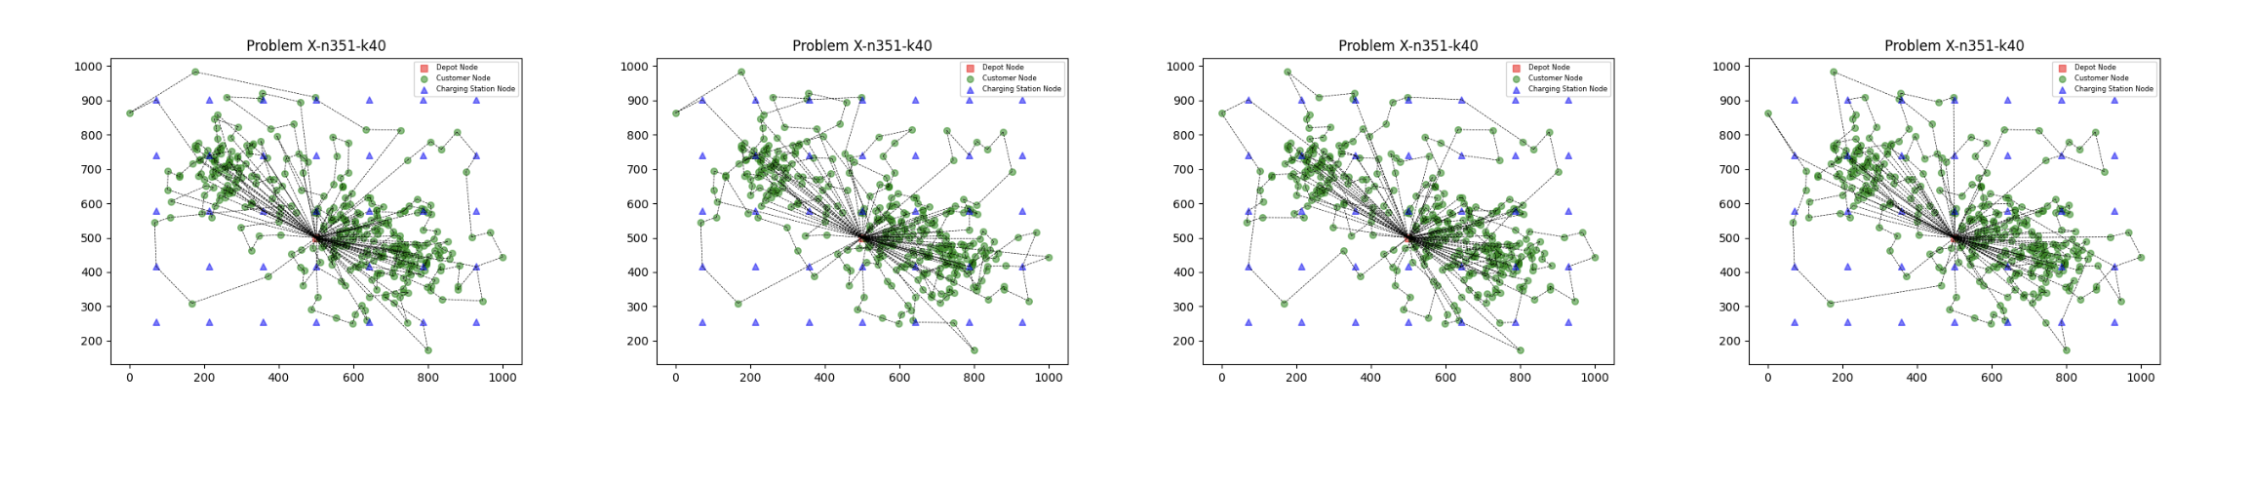
\includegraphics[width=\textwidth]{image/4/final/351-40.png}
    \caption{Solution visualization for \textbf{X-n352-k40.evrp}. From left to right: Greedy Search, GA, SA, and ACO.}
    \label{fig:solution-xn352k40}
\end{figure}

\begin{figure}[!h]
    \centering
    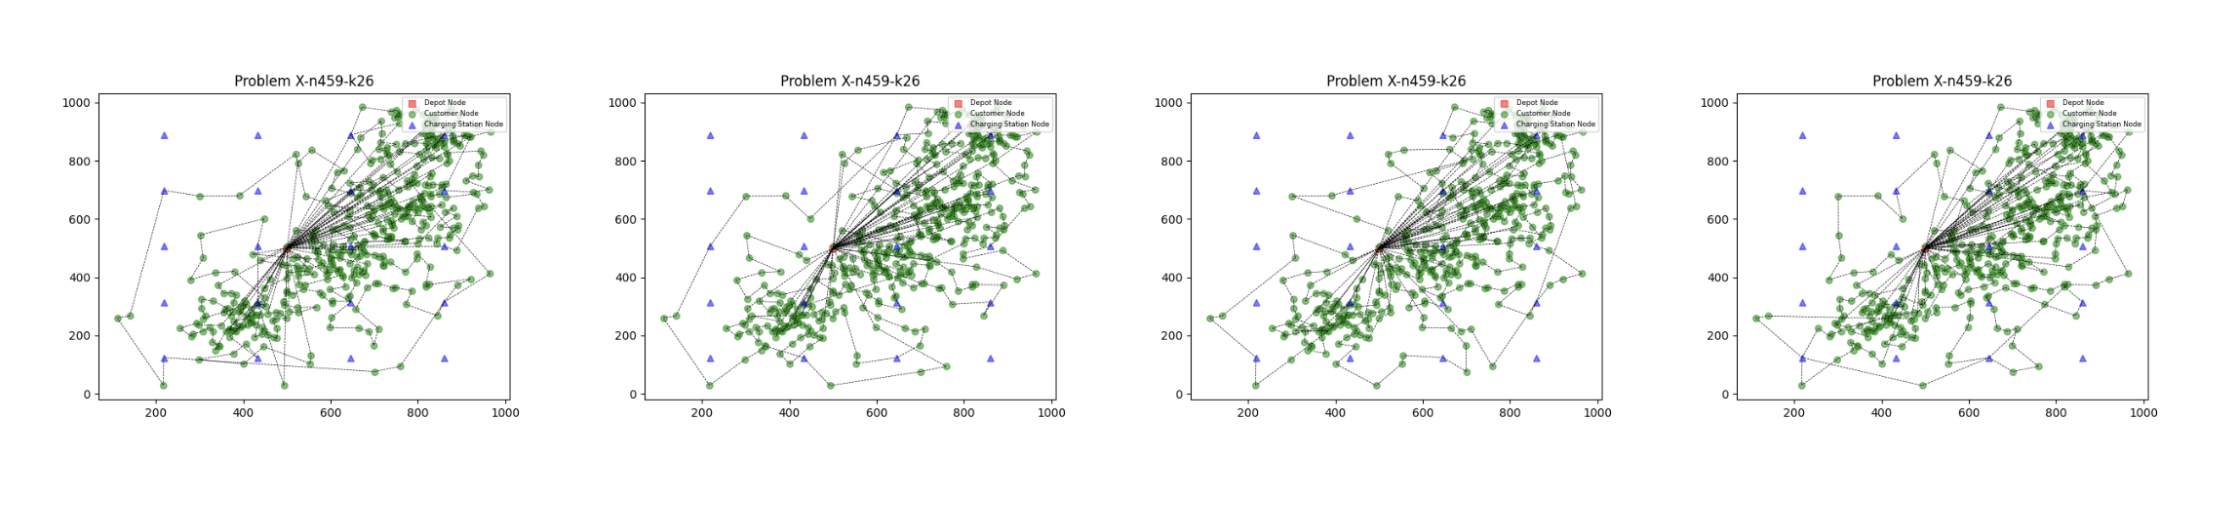
\includegraphics[width=\textwidth]{image/4/final/459-26.png}
    \caption{Solution visualization for \textbf{X-n459-k26.evrp}. From left to right: Greedy Search, GA, SA, and ACO.}
    \label{fig:solution-xn459k26}
\end{figure}

\begin{figure}[!h]
    \centering
    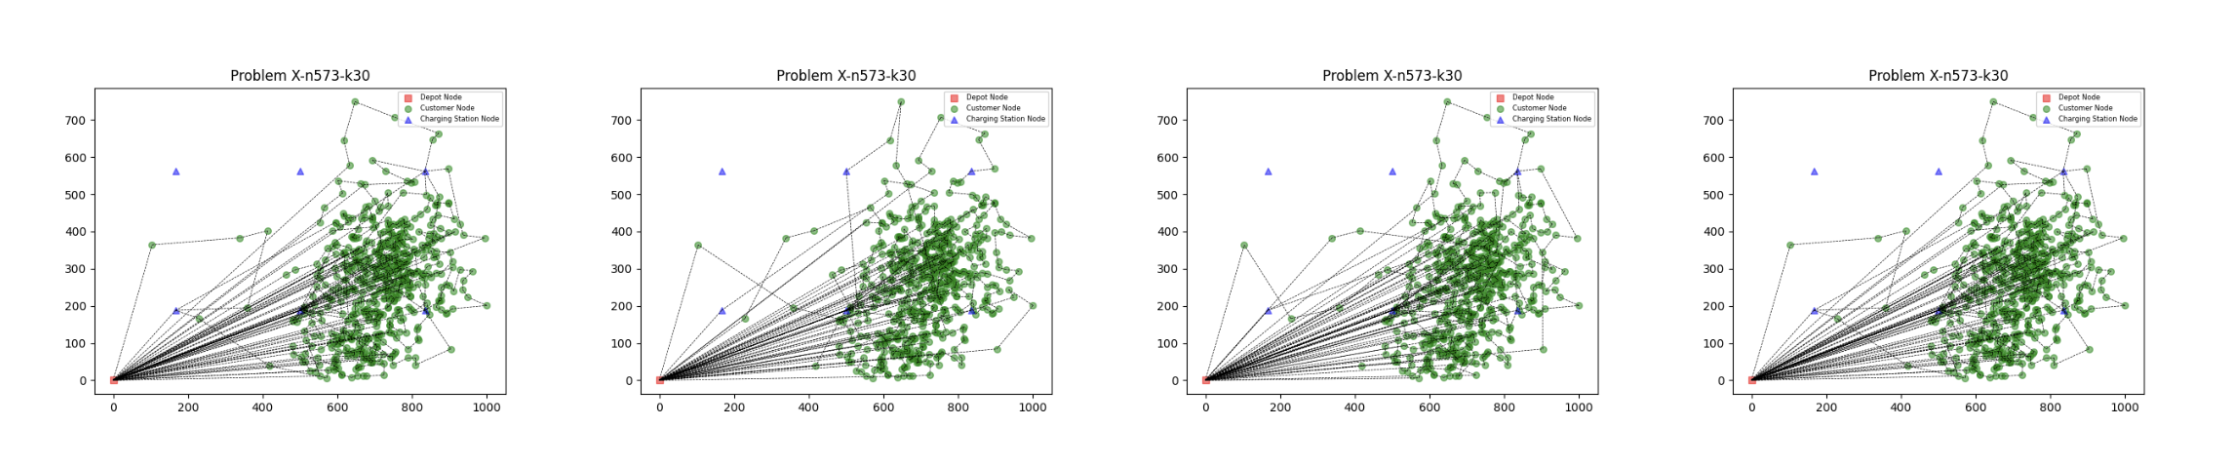
\includegraphics[width=\textwidth]{image/4/final/573-30.png}
    \caption{Solution visualization for \textbf{X-n573-k30.evrp}. From left to right: Greedy Search, GA, SA, and ACO.}
    \label{fig:solution-xn573k30}
\end{figure}

\begin{figure}[!h]
    \centering
    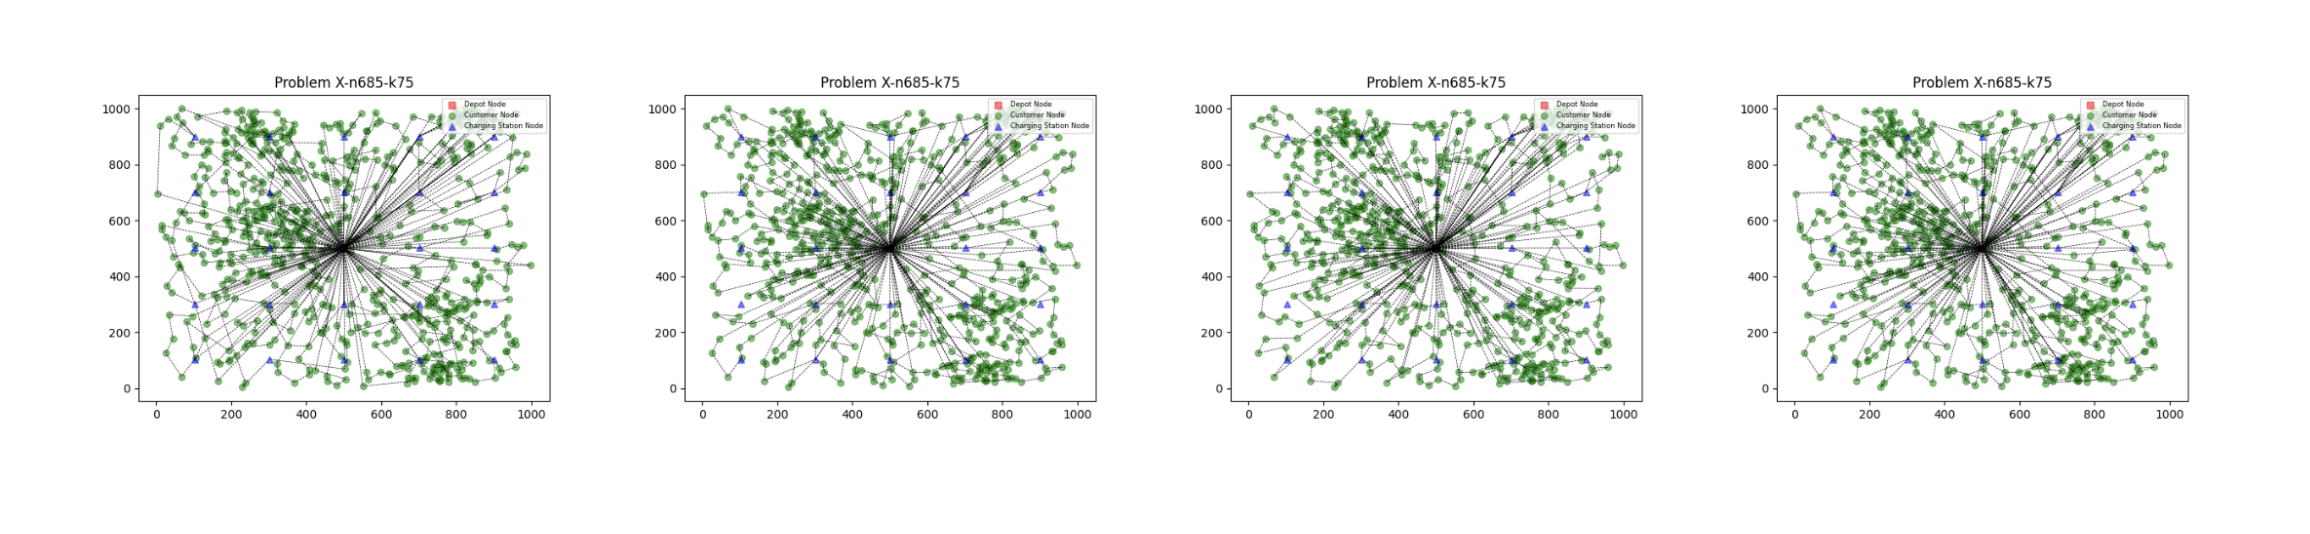
\includegraphics[width=\textwidth]{image/4/final/658-75.png}
    \caption{Solution visualization for \textbf{X-n685-k75.evrp}. From left to right: Greedy Search, GA, SA, and ACO.}
    \label{fig:solution-xn685k75}
\end{figure}
From the visualizations, several consistent patterns can be observed:

First, it is clear that the second plot (corresponding to GA) and the fourth plot (corresponding to SA) typically exhibit the most organized and efficient routing structures.
The vehicle paths generated by GA and SA cover all customers systematically, minimize unnecessary detours, and display smooth transitions between depot visits and customer services.
In contrast, the paths generated by the baseline Greedy Search often appear chaotic, with irregular loops, frequent returns to the depot, and missed opportunities for efficient clustering of nearby customers.
This phenomenon becomes particularly pronounced in large-scale instances (e.g., X-n573-k30, X-n685-k75), where the Greedy approach struggles to maintain any coherent tour structure.

Second, GA consistently produces the most compact and logical routes.
The tours are well clustered, respect energy and capacity constraints, and exhibit minimal redundancy in movement.
This confirms GA’s strong ability to balance global exploration and local refinement through its perturbation-driven evolutionary operators.

Third, although ACO generally performs well, some of its solutions show slight zigzagging or excessive charging station visits compared to GA.
This suggests that while pheromone guidance helps structure the search, it may occasionally lead to over-exploration when energy constraints dominate the decision-making process.

Fourth, SA's performance is mixed: on smaller instances (e.g., E-n22-k4, E-n23-k3), SA produces highly competitive and neat routes, closely matching GA.
However, on larger instances (e.g., X-n351-k40, X-n573-k30), SA solutions exhibit greater irregularities, including fragmented customer servicing and higher reliance on charging stations, reflecting the instability issues discussed in the quantitative analysis.

\subsection{Parameter Sensitivity Analysis }
\begin{figure}[!h]
    \centering
    \begin{tabular}{ccc}
        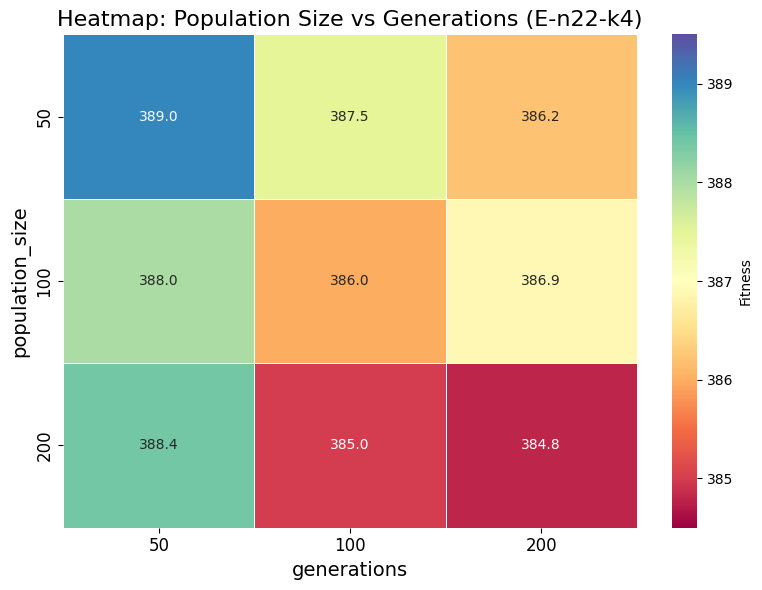
\includegraphics[width=0.3\textwidth]{image/4/parameter/ga/22_4.png} &
        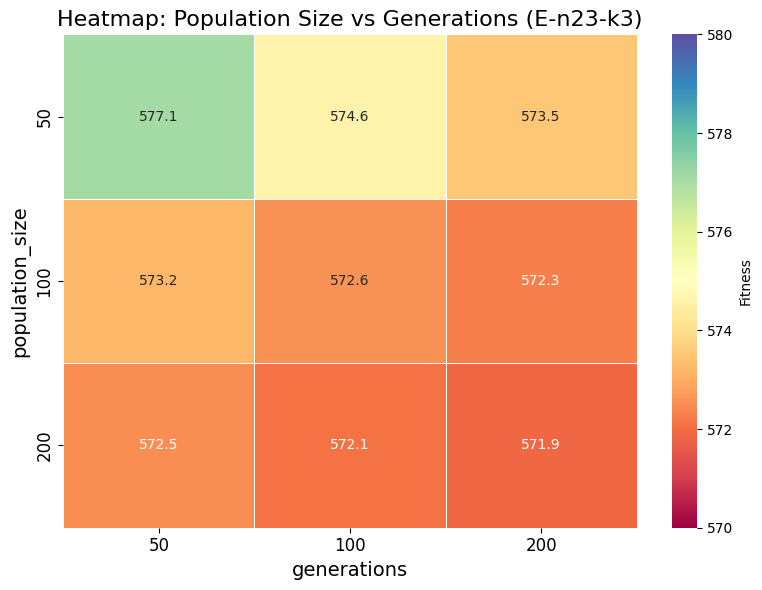
\includegraphics[width=0.3\textwidth]{image/4/parameter/ga/23_3.png} &
        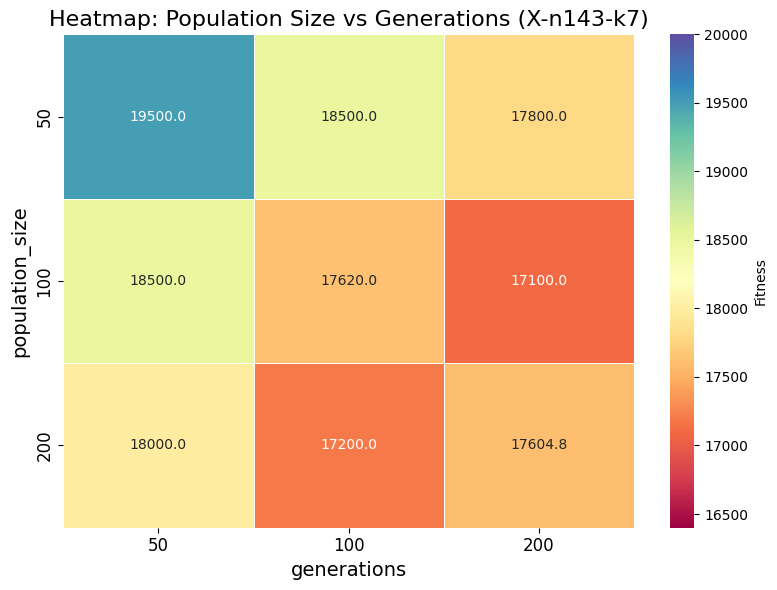
\includegraphics[width=0.3\textwidth]{image/4/parameter/ga/143_7.png} \\
        \small (a) E-n22-k4.evrp & \small (b) E-n23-k3.evrp & \small (c) X-n143-k7.evrp \\
        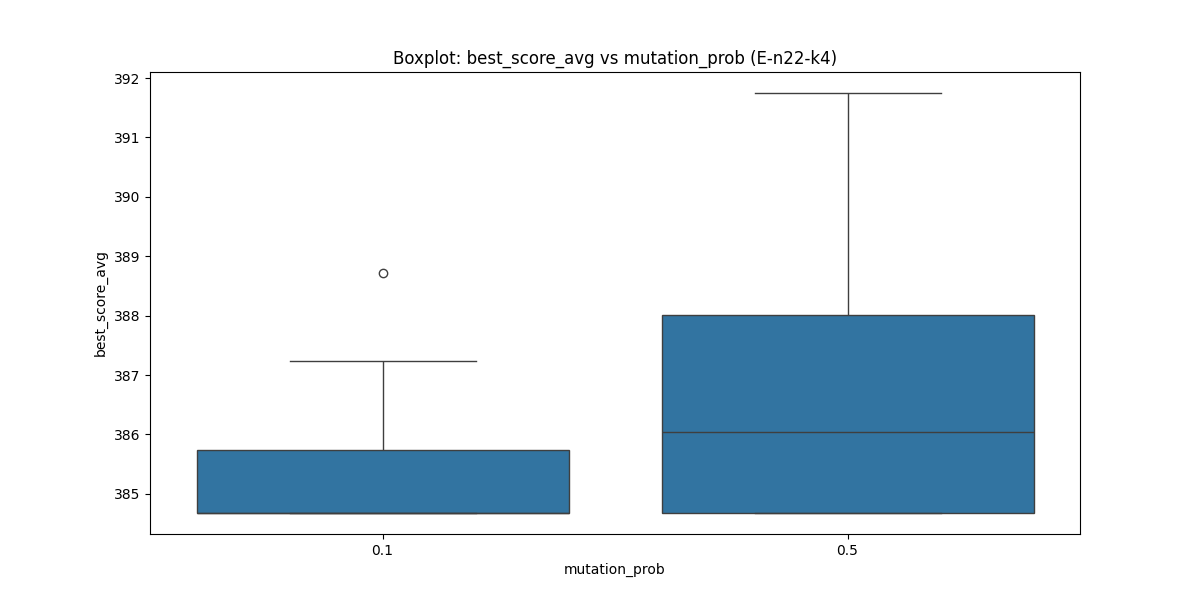
\includegraphics[width=0.4\textwidth]{image/4/parameter/ga/E-n22-k4_boxplot_mutation_prob.png} &
        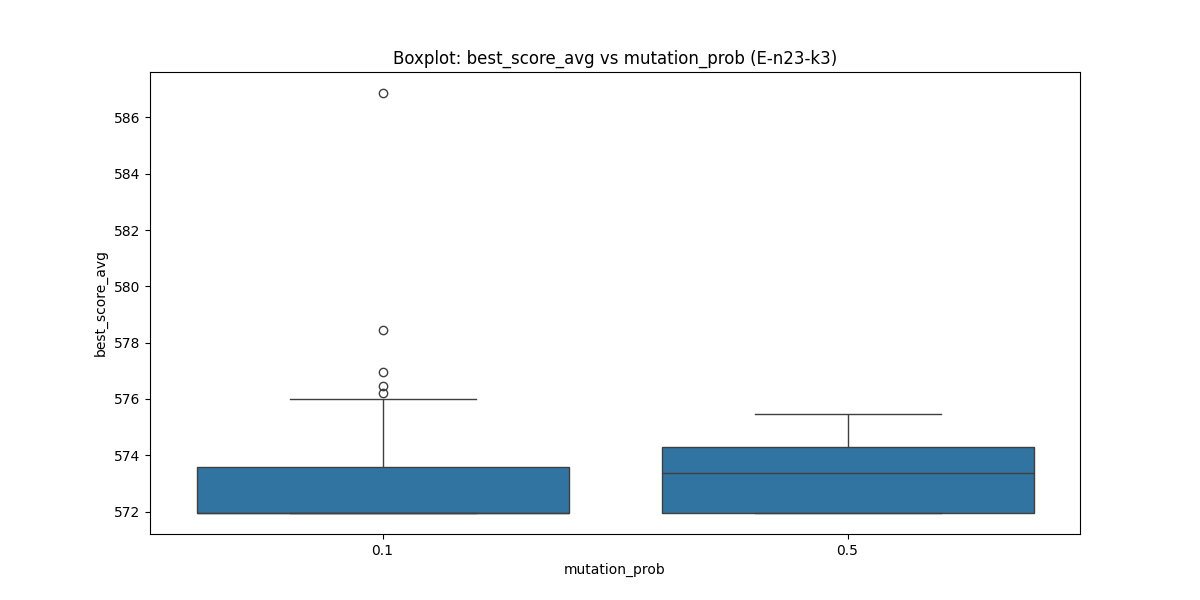
\includegraphics[width=0.4\textwidth]{image/4/parameter/ga/E-n23-k3_boxplot_mutation_prob.png} & \\
        \small (d) E-n22-k4.evrp & \small (e) E-n23-k3.evrp & \\
    \end{tabular}
    \caption{(Top) Heatmaps of performance under different GA settings; (Bottom) Boxplots of mutation probability effects for GA on selected EVRP instances.}
    \label{fig:ga-parameter-analysis}
\end{figure}
\paragraph{Parameter Analysis for GA.}
Figure~\ref{fig:ga-parameter-analysis} provides an in-depth visualization of how key Genetic Algorithm (GA) parameters affect the performance on the EVRP benchmark.

Firstly, the heatmaps (a–c) demonstrate that increasing the population size and the number of generations consistently leads to improved solution quality, as indicated by lower fitness values.  
A larger population size enhances the diversity of the genetic pool, promoting broader exploration of the search space and reducing the risk of premature convergence.  
Simultaneously, a greater number of generations provides the algorithm with more opportunities to refine solutions through selection, crossover, and mutation processes.  
However, the benefits of increasing these parameters exhibit diminishing returns beyond certain thresholds, particularly when moving from moderate to very large values.  
This suggests that while promoting diversity and iterative refinement is critical, excessively large settings may introduce significant computational overhead without commensurate gains in solution quality.

Secondly, the boxplots (d–e) examine the effects of different mutation probabilities.  
For the \textit{E-n22-k4} instance, a lower mutation rate (0.1) yields more concentrated and stable fitness distributions, suggesting that limited yet controlled random perturbations are sufficient to guide the search effectively in smaller-scale problems.  
Conversely, for the \textit{E-n23-k3} instance, a mutation probability of 0.5 slightly improves performance, implying that greater exploration is advantageous in more complex search landscapes to escape local optima.  
These observations indicate that the optimal mutation intensity is instance-dependent: lower mutation rates promote convergence stability, whereas higher rates enhance exploration in rugged solution spaces.

Overall, these findings highlight the complementary roles of each GA parameter:

\begin{itemize}
    \item \textbf{Population Size}: Governs genetic diversity and global exploration capacity; larger sizes enhance exploration but with diminishing returns beyond a certain point.
    \item \textbf{Number of Generations}: Determines evolutionary depth; more generations enable deeper refinement of solutions.
    \item \textbf{Mutation Probability}: Balances exploration and exploitation; lower rates stabilize convergence, while higher rates encourage escaping local optima.
\end{itemize}

Careful tuning of these parameters ensures that the Genetic Algorithm maintains a robust balance between exploration and exploitation, ultimately achieving high-quality and stable solutions across diverse EVRP instances.

\begin{figure}[!h]
    \centering
    \begin{tabular}{ccc}
        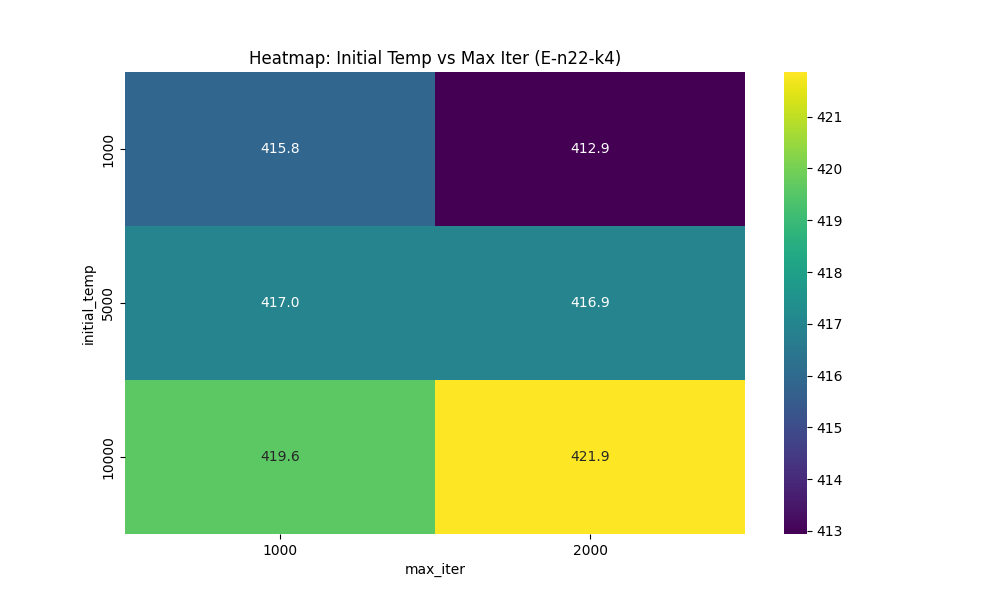
\includegraphics[width=0.3\textwidth]{image/4/parameter/sa/E-n22-k4_heatmap_temp_iter.png} &
        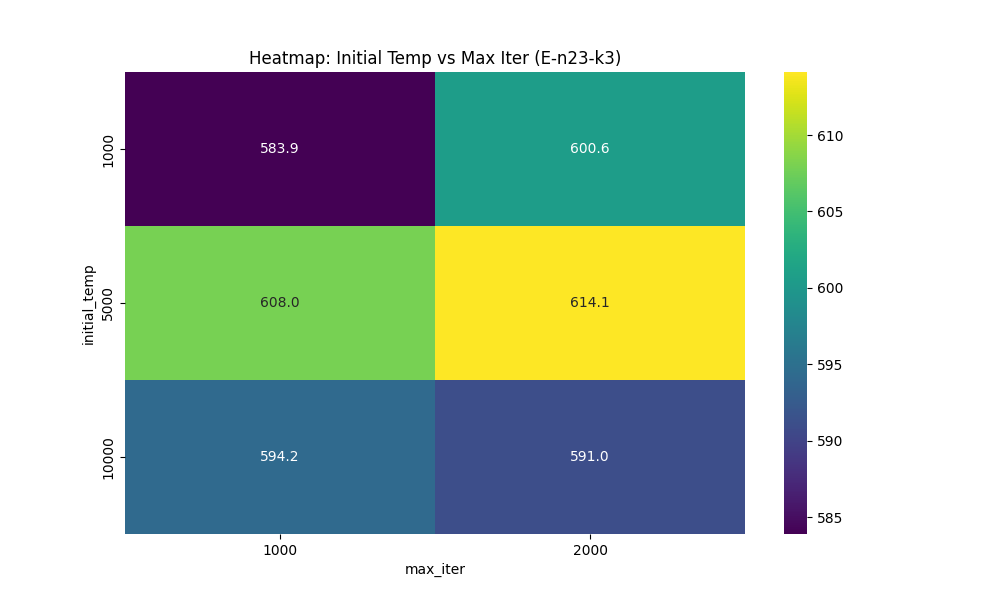
\includegraphics[width=0.3\textwidth]{image/4/parameter/sa/E-n23-k3_heatmap_temp_iter.png} &
        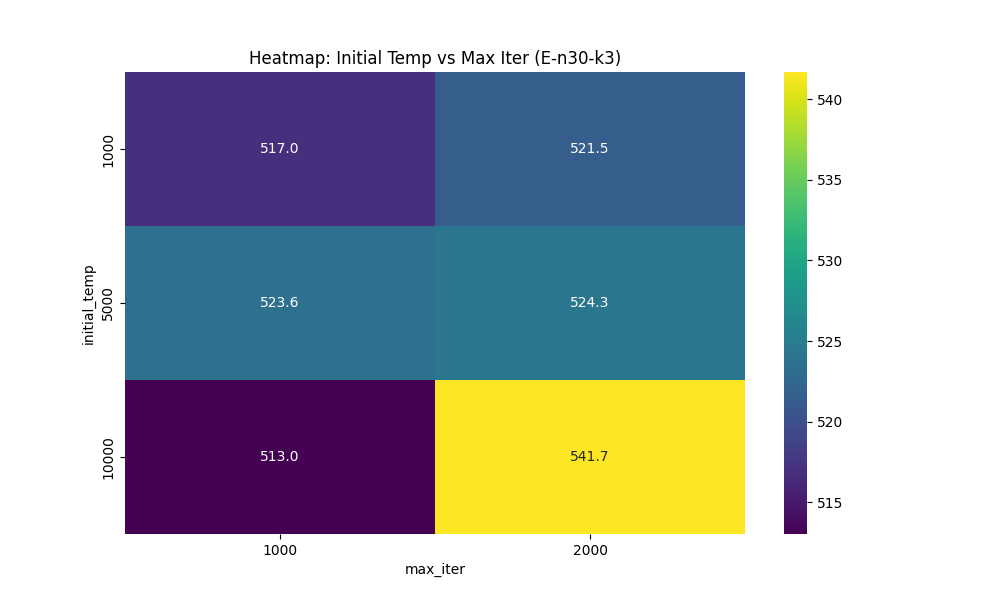
\includegraphics[width=0.3\textwidth]{image/4/parameter/sa/E-n30-k3_heatmap_temp_iter.png} \\
        \small (a) E-n22-k4.evrp & \small (b) E-n23-k3.evrp & \small (c) E-n30-k3.evrp \\
        
        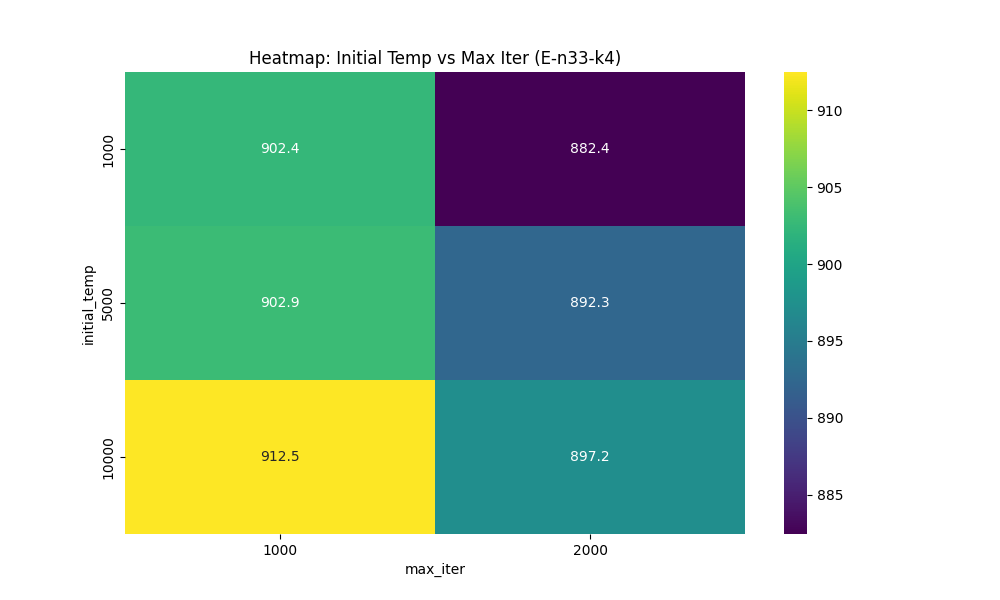
\includegraphics[width=0.3\textwidth]{image/4/parameter/sa/E-n33-k4_heatmap_temp_iter.png} &
        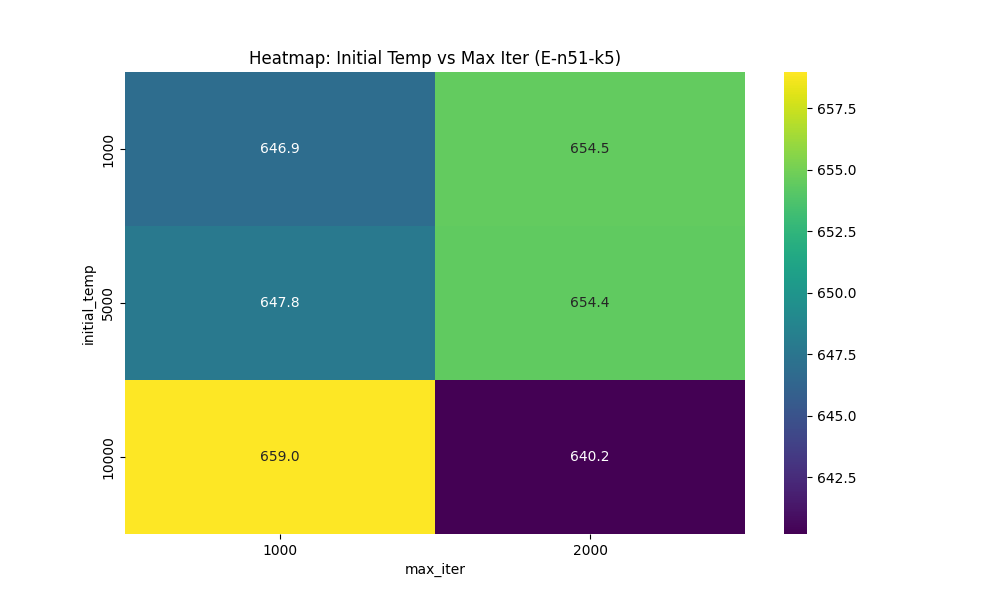
\includegraphics[width=0.3\textwidth]{image/4/parameter/sa/E-n51-k5_heatmap_temp_iter.png} &
        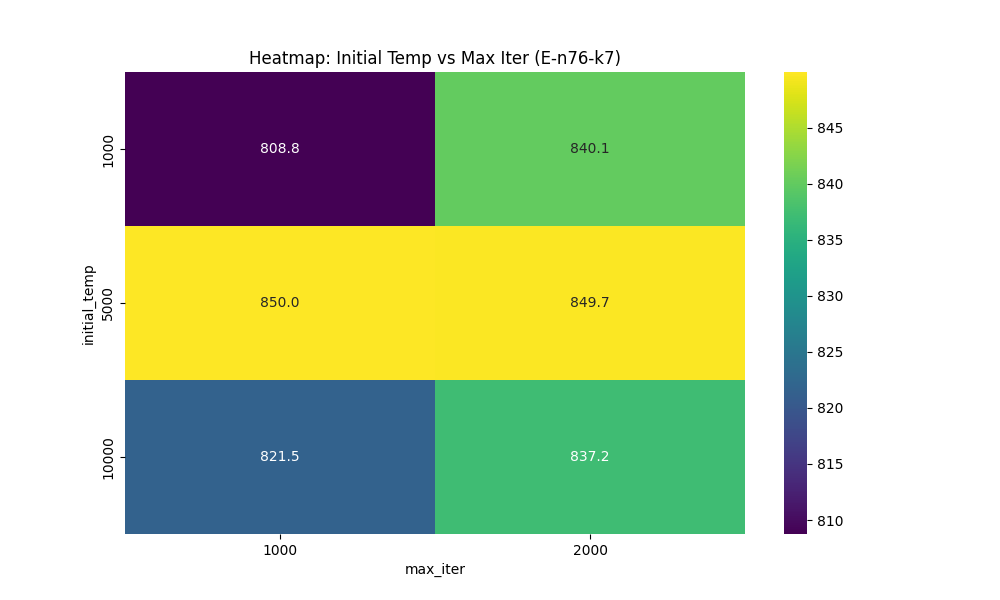
\includegraphics[width=0.3\textwidth]{image/4/parameter/sa/E-n76-k7_heatmap_temp_iter.png} \\
        \small (d) E-n33-k4.evrp & \small (e) E-n51-k5.evrp & \small (f) E-n76-k7.evrp \\
        
        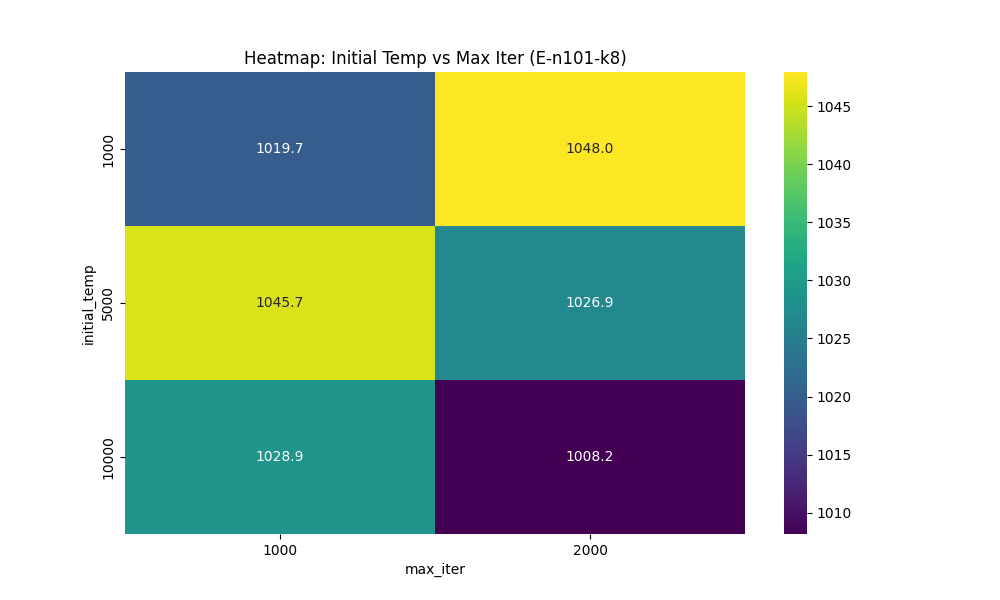
\includegraphics[width=0.3\textwidth]{image/4/parameter/sa/E-n101-k8_heatmap_temp_iter.png} &
        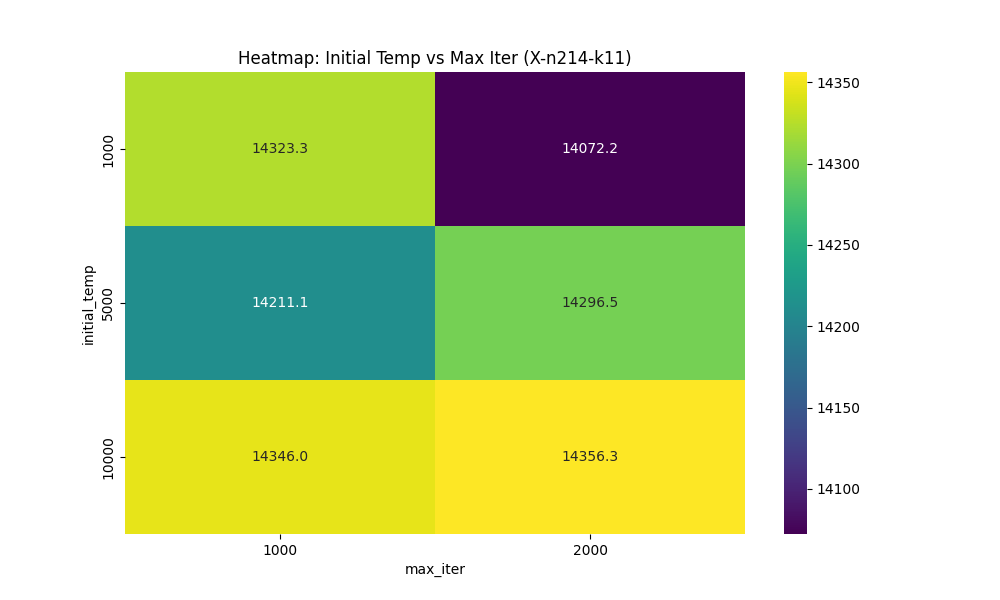
\includegraphics[width=0.3\textwidth]{image/4/parameter/sa/X-n214-k11_heatmap_temp_iter.png} &
        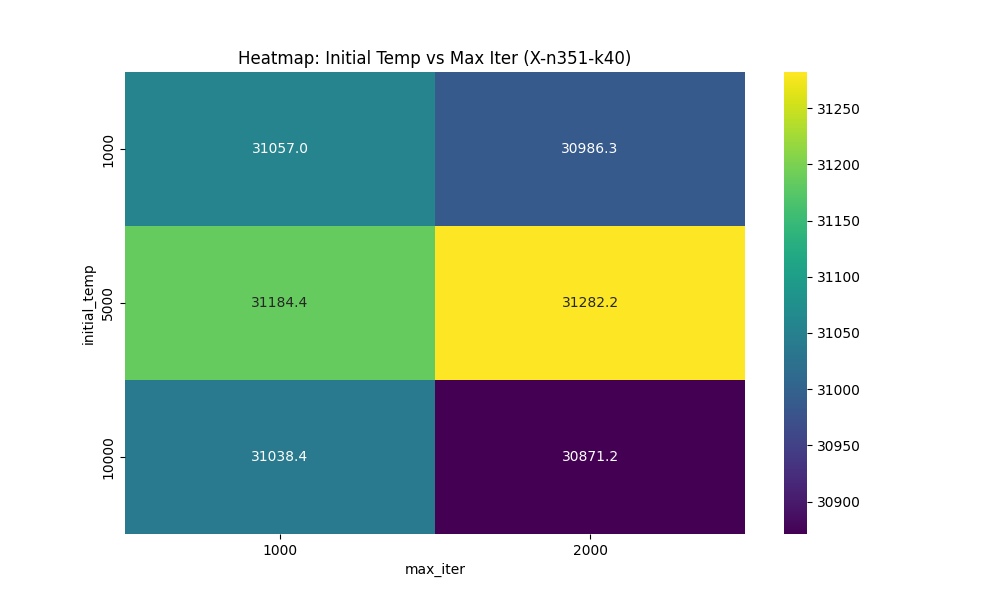
\includegraphics[width=0.3\textwidth]{image/4/parameter/sa/X-n351-k40_heatmap_temp_iter.png} \\
        \small (g) E-n101-k8.evrp & \small (h) X-n214-k11.evrp & \small (i) X-n351-k40.evrp \\
    \end{tabular}
    \caption{Parameter sensitivity analysis on Simulated Annealing (SA) over different EVRP instances.}
    \label{fig:sa-parameter-heatmaps}
\end{figure}
\noindent
\paragraph{Parameter Sensitivity Analysis for SA.}
Figure~\ref{fig:sa-parameter-heatmaps} illustrates the impact of \textbf{initial temperature} and \textbf{maximum iterations} on the performance of Simulated Annealing (SA) across various EVRP instances.

Overall, increasing the \textbf{maximum number of iterations} consistently improves solution quality by enabling more thorough exploration of the search space, particularly for smaller instances such as \textit{E-n22-k4} and \textit{E-n33-k4}.  
However, for moderately complex instances like \textit{E-n30-k3} and large-scale instances such as \textit{X-n351-k40}, the marginal gains from additional iterations diminish, suggesting the existence of a computational efficiency-saturation point.

The role of \textbf{initial temperature} appears to be more instance-dependent.  
For smaller problems, setting a \textbf{lower initial temperature} facilitates faster convergence by limiting unnecessary random exploration in early search phases, leading to quicker stabilization and lower final fitness values.  
In contrast, for larger-scale instances such as \textit{X-n214-k11}, the influence of the initial temperature is less significant, indicating that extensive search iterations are more crucial than initial exploration intensity.


\begin{figure}[!h]
    \centering
    \begin{tabular}{cccc}
        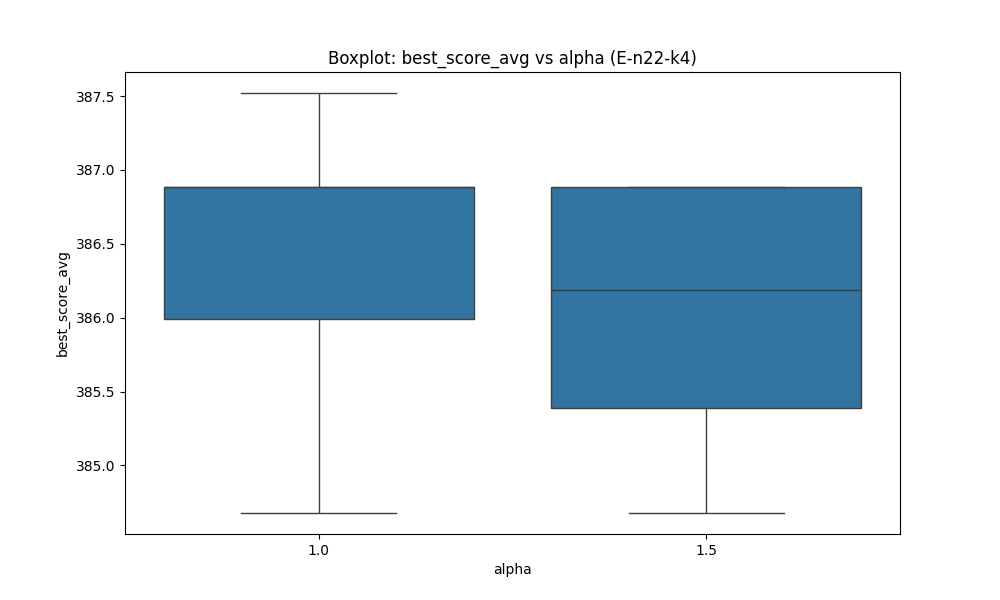
\includegraphics[width=0.22\textwidth]{image/4/parameter/aco/E-n22-k4_boxplot_alpha.png} &
        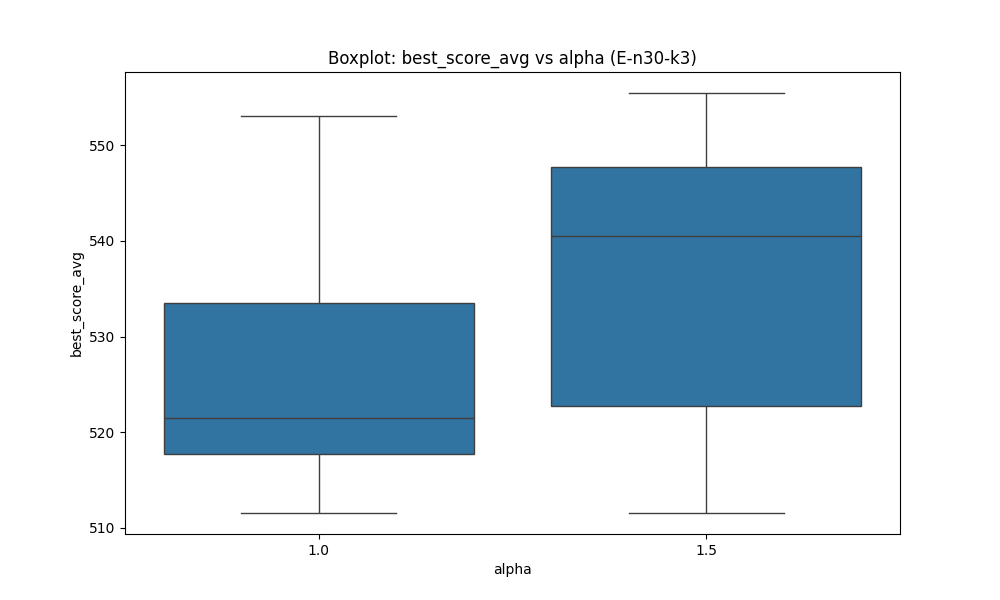
\includegraphics[width=0.22\textwidth]{image/4/parameter/aco/E-n30-k3_boxplot_alpha.png} &
        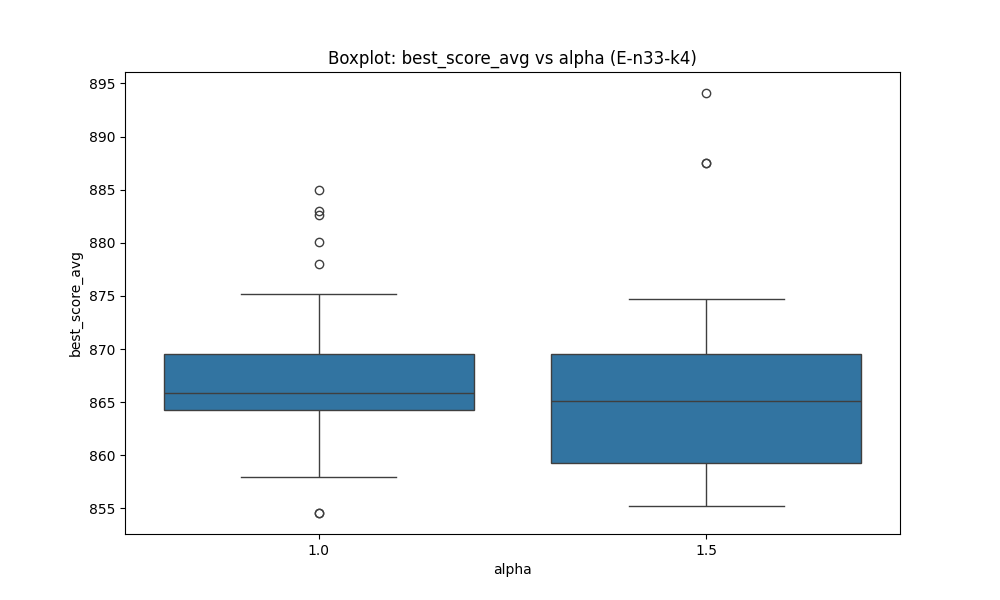
\includegraphics[width=0.22\textwidth]{image/4/parameter/aco/E-n33-k4_boxplot_alpha.png} &
        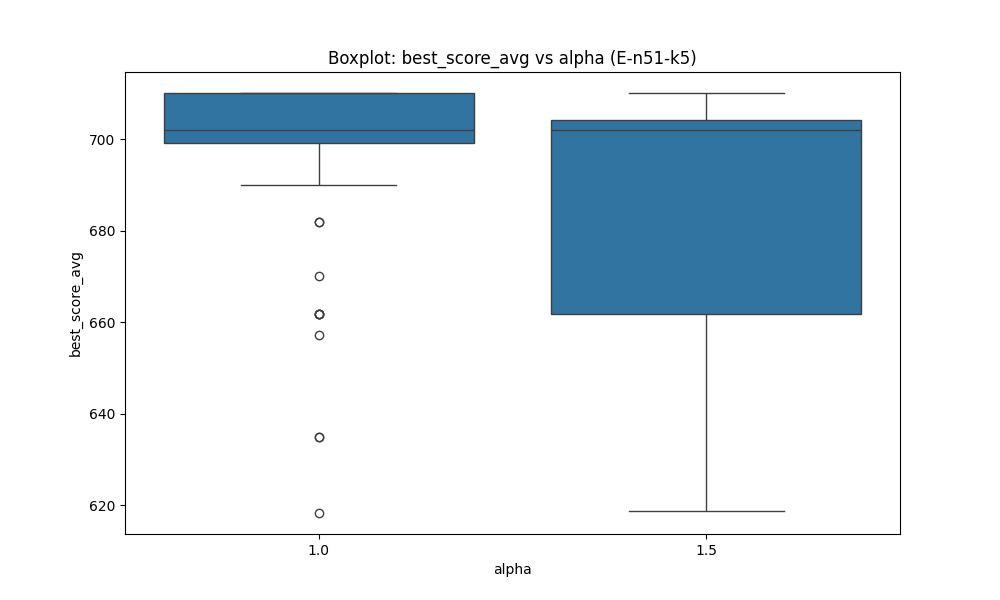
\includegraphics[width=0.22\textwidth]{image/4/parameter/aco/E-n51-k5_boxplot_alpha.png} \\
        \small (a) E-n22-k4.evrp & \small (b) E-n30-k3.evrp & \small (c) E-n33-k4.evrp & \small (d) E-n51-k5.evrp \\
        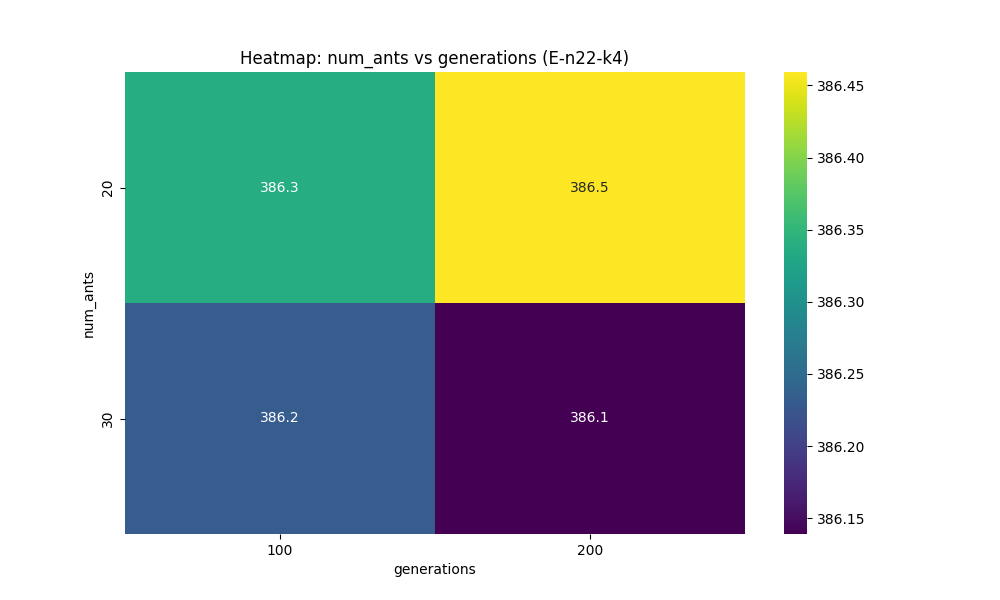
\includegraphics[width=0.22\textwidth]{image/4/parameter/aco/E-n22-k4_heatmap_ants_gen.png} &
        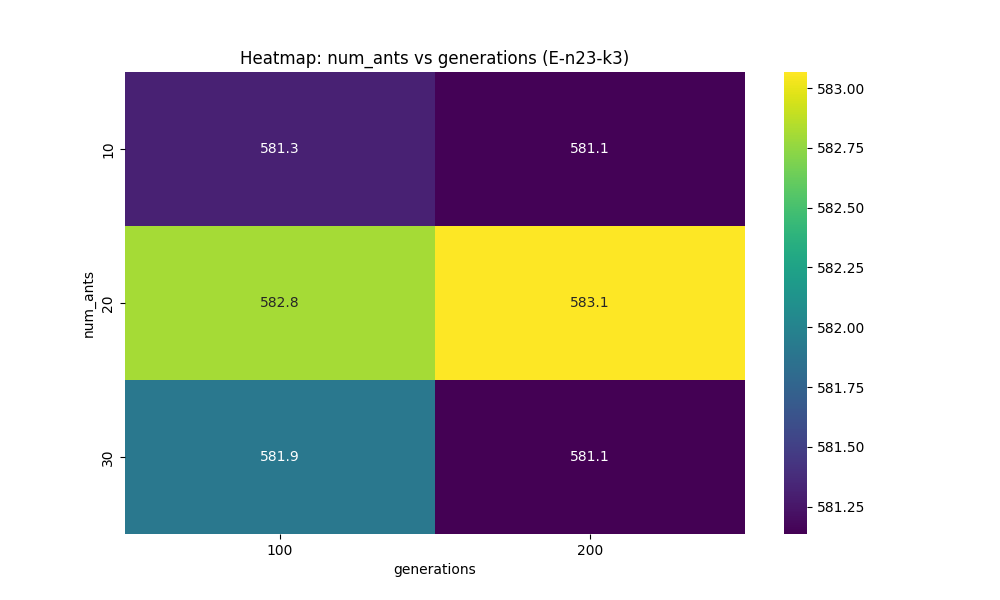
\includegraphics[width=0.22\textwidth]{image/4/parameter/aco/E-n23-k3_heatmap_ants_gen.png} &
        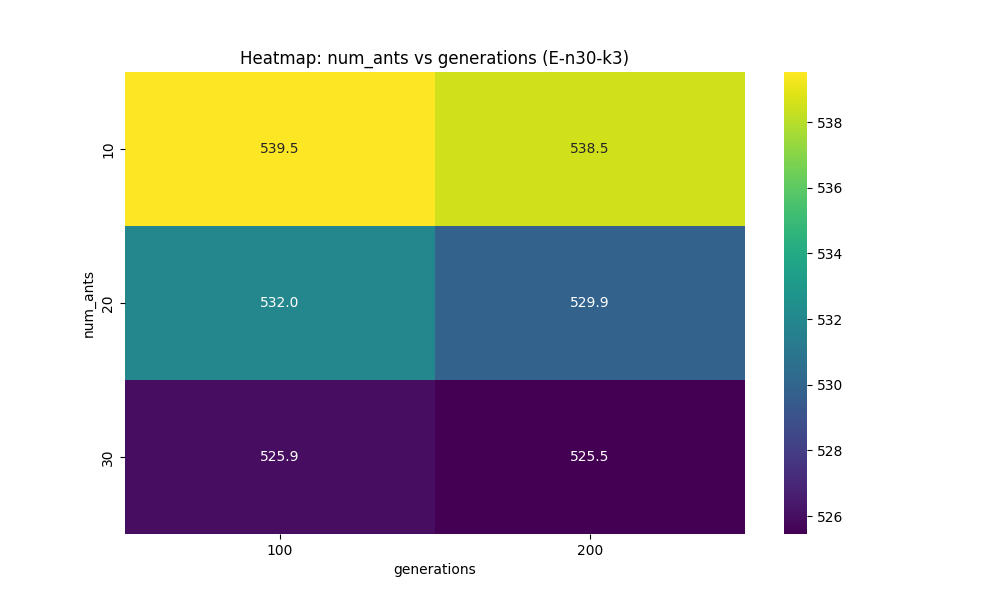
\includegraphics[width=0.22\textwidth]{image/4/parameter/aco/E-n30-k3_heatmap_ants_gen.png} &
        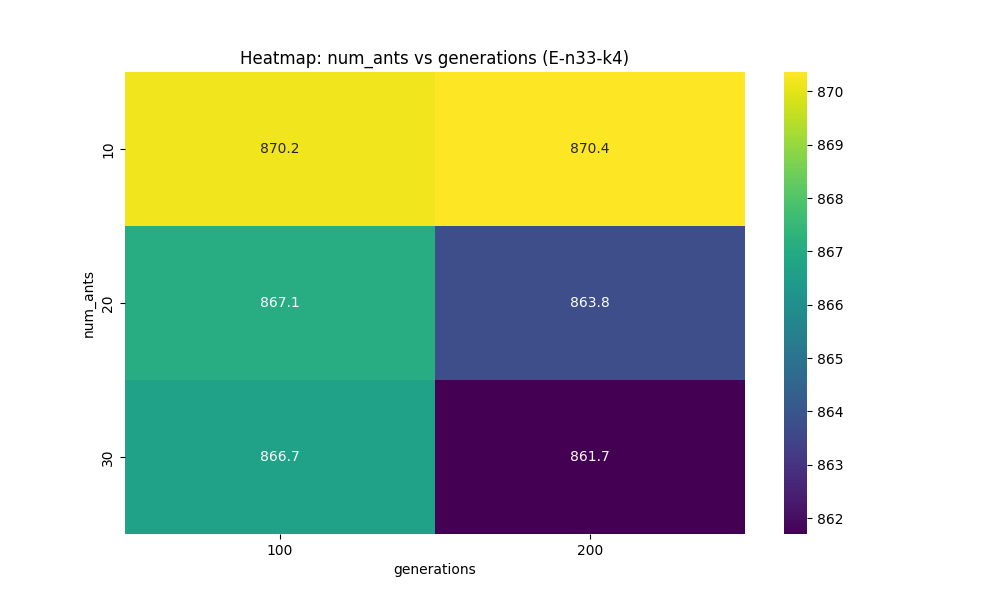
\includegraphics[width=0.22\textwidth]{image/4/parameter/aco/E-n33-k4_heatmap_ants_gen.png} \\
        \small (e) E-n22-k4.evrp & \small (f) E-n23-k3.evrp & \small (g) E-n30-k3.evrp & \small (h) E-n33-k4.evrp \\
    \end{tabular}
    \caption{(Top) Boxplots of different $\alpha$ values in ACO; (Bottom) Heatmaps of ant numbers vs generations for ACO parameter sensitivity analysis on selected EVRP instances.}
    \label{fig:aco-parameter-analysis}
\end{figure}
\noindent
\paragraph{Parameter Sensitivity Analysis for ACO.}
Figure~\ref{fig:aco-parameter-analysis} presents the sensitivity analysis of Ant Colony Optimization (ACO) parameters on selected EVRP instances.

The boxplots (a--d) show the influence of different $\alpha$ values, which control the relative importance of pheromone trails during solution construction. 
On smaller instances such as \textit{E-n22-k4} and \textit{E-n30-k3}, increasing $\alpha$ from 1.0 to 1.5 slightly improves solution quality, indicating that stronger pheromone guidance accelerates convergence.
However, for larger instances like \textit{E-n51-k5}, a higher $\alpha$ introduces greater solution variability, suggesting that excessive pheromone reliance can lead to premature convergence and instability.

The heatmaps (e--h) illustrate the impact of varying the number of ants and generations.
In general, increasing both parameters improves solution quality, particularly on medium-scale instances like \textit{E-n30-k3} and \textit{E-n33-k4}.
Nevertheless, for certain cases such as \textit{E-n23-k3}, increasing the number of ants beyond a threshold does not yield consistent improvements, implying that search redundancy may counteract exploration benefits.
\section{Discussion}
\label{sec:discussion}

The comprehensive experimental results provide several important insights into the effectiveness, robustness, and scalability of the proposed perturbation-driven metaheuristic algorithms for solving the Electric Vehicle Routing Problem (EVRP).

\subsection{Substantial Improvements over Greedy Baseline}
Across all instances, the Greedy Search baseline exhibits significantly higher mean tour lengths and larger standard deviations compared to the proposed algorithms (GA, ACO, SA). 
This confirms that the integration of structured perturbations and local search modules dramatically improves both solution quality and robustness.
The improvement remains consistent across small, medium, and large-scale instances, demonstrating that simple greedy heuristics are insufficient for handling the complex energy and load constraints inherent in EVRP.

\subsection{Effectiveness Hierarchy: GA $>$ ACO $>$ SA}
Among the metaheuristics, GA consistently achieves the best performance, followed by ACO and then SA. 
GA not only yields the lowest best, mean, and maximum fitness values, but also maintains the highest stability (smallest standard deviation) across all instances.
This validates the advantage of GA’s design, which balances global exploration and local refinement through adaptive crossover, mutation, and local search strategies.  
ACO benefits from pheromone-guided search and delivers stable results but is still slightly less effective due to limited adaptability under dynamic constraints.
SA exhibits the largest performance variability, particularly on large-scale instances, reflecting the risk of local minima entrapment in purely temperature-driven exploration.

\subsection{Scalability to Large-Scale Instances}
As the instance size increases (e.g., X-n573-k30, X-n685-k75), all algorithms experience natural degradation in solution quality and stability.
However, the relative ranking remains unchanged: GA continues to outperform ACO and SA, demonstrating superior scalability.
This indicates that the perturbation-driven design principles generalize well even under extreme problem sizes and complexity.

\subsection{Qualitative Analysis Confirms Solution Rationality}
The solution visualizations further validate the quantitative findings.  
GA and SA solutions exhibit well-structured, logical, and compact routing patterns, systematically covering all customers while minimizing redundant paths and excessive charging visits. 
Greedy solutions, in contrast, show chaotic, fragmented tours with frequent depot returns.
ACO solutions are reasonably organized but sometimes suffer from slight over-exploration due to heavy pheromone reliance.

\subsection{Parameter Sensitivity Reveals Key Design Principles}
The parameter sensitivity analysis reveals that:
\begin{itemize}
    \item For \textbf{GA}, larger population sizes and more generations generally enhance performance, while moderate mutation probabilities strike a better balance between exploration and convergence.
    \item For \textbf{SA}, increasing the number of iterations consistently improves solutions, while tuning the initial temperature is important for small to medium problems.
    \item For \textbf{ACO}, carefully balancing pheromone importance ($\alpha$) and controlling the number of ants and generations is crucial; overly strong pheromone influence or excessive ants can destabilize performance.
\end{itemize}
These observations emphasize the necessity of fine-tuning search parameters based on problem scale and characteristics to achieve optimal results.

\paragraph{Impact of Code Design Enhancements.}
The superior performance of all three algorithms is further attributed to the algorithmic enhancements incorporated into the codebase:
\begin{itemize}
    \item The adoption of \textbf{iterated 2-opt} and \textbf{3-opt} local search ensures strong intra-route optimization.
    \item The introduction of \textbf{perturbation mechanisms} (e.g., adaptive mutation in GA, layered pheromone perturbation in ACO, reheating in SA) enhances global exploration while maintaining feasible solutions.
\end{itemize}

